\documentclass[11pt,a4paper,oneside]{report}

\usepackage[utf8]{inputenc}
\usepackage[T1]{fontenc}
\usepackage[turkish]{babel}

\usepackage[margin=2.2cm]{geometry}
\usepackage{graphicx}
\usepackage{xcolor}
\usepackage{titlesec}
\usepackage{fancyhdr}
\usepackage{hyperref}
\usepackage{listings}
\usepackage{tikz}
\usepackage{tcolorbox}
\tcbuselibrary{skins}
\usepackage{array}
\usepackage{booktabs}
\usepackage{caption}
\usepackage{fontawesome5}

\definecolor{primary}{RGB}{50, 50, 50}
\definecolor{secondary}{RGB}{100, 100, 100}
\definecolor{linkblue}{RGB}{31, 78, 121}
\definecolor{darkgray}{RGB}{45, 52, 54}
\definecolor{lightgray}{RGB}{245, 247, 250}
\definecolor{bordergray}{RGB}{200, 205, 210}
\definecolor{codeblue}{RGB}{45, 85, 125}
\definecolor{codegreen}{RGB}{80, 120, 90}
\definecolor{codered}{RGB}{160, 60, 60}

\hypersetup{
    colorlinks=true,
    linkcolor=linkblue,
    filecolor=linkblue,
    urlcolor=linkblue,
    citecolor=linkblue
}

\setlength{\headheight}{23pt}
\pagestyle{fancy}
\fancyhf{}
\lhead{\small \bfseries \textcolor{primary}{\leftmark}}
\rhead{\small \textcolor{secondary}{Excel Uygulama Raporu}}
\cfoot{\small \bfseries \textcolor{primary}{\thepage}}
\renewcommand{\headrulewidth}{0.8pt}
\renewcommand{\headrule}{\hbox to\headwidth{\color{primary}\linewidth 0.8pt\hss}}

\titleformat{\chapter}[block]
  {\normalfont\huge\bfseries\color{primary}}
  {\tcbset{sharp corners}
   \begin{tcolorbox}[colback=primary,colframe=primary,arc=0pt,top=4pt,bottom=4pt,left=8pt,right=8pt,before upper=\strut]
     \textcolor{white}{\thechapter}
   \end{tcolorbox}\ }
  {0.5em}
  {}
\titlespacing*{\chapter}{0pt}{0pt}{20pt}
  
\titleformat{\section}
  {\normalfont\Large\bfseries\color{primary}}{\thesection}{0.8em}{}
  
\titleformat{\subsection}
  {\normalfont\large\bfseries\color{secondary}}{\thesubsection}{0.8em}{}

\lstdefinelanguage{VBA}{
  morekeywords={
    Attribute, VB_Name, Option, Explicit, Public, Private, Sub, End, Function,
    Dim, As, Set, New, For, Each, In, Next, If, Then, Else, ElseIf, Select, Case,
    With, Exit, True, False, Long, String, Integer, Boolean, Variant, Object, Collection,
    Worksheet, Range, Workbook, On, Error, GoTo, Resume, ReDim, Split, Val, CStr, CInt, CDate
  },
  sensitive=false,
  morecomment=[l]{'},
  morestring=[b]"
}

\lstset{
  language=VBA,
  backgroundcolor=\color{lightgray},
  basicstyle=\ttfamily\footnotesize\color{darkgray},
  breaklines=true,
  captionpos=b,
  commentstyle=\color{codegreen}\itshape,
  keywordstyle=\color{codeblue}\bfseries,
  stringstyle=\color{codered},
  numbers=left,
  numberstyle=\tiny\color{gray},
  numbersep=10pt,
  frame=leftline,
  framerule=3pt,
  rulecolor=\color{primary},
  tabsize=4,
  showstringspaces=false,
  extendedchars=true,
  inputencoding=utf8,
  literate={ç}{{\c{c}}}1 {ğ}{{\u{g}}}1 {ı}{{\i}}1 {İ}{{\.{I}}}1 {ö}{{\"o}}1 {ş}{{\c{s}}}1 {ü}{{\"u}}1
           {Ç}{{\c{C}}}1 {Ğ}{{\u{G}}}1 {Ö}{{\"O}}1 {Ş}{{\c{S}}}1 {Ü}{{\"U}}1
}

\tcbset{
  sharp corners,
  enhanced,
  boxrule=0pt
}

\newtcolorbox{warningbox}[1]{
  colback=black!4!white,
  colframe=primary,
  leftrule=4pt,
  fonttitle=\bfseries\color{primary},
  title=#1,
  coltitle=primary,
  colbacktitle=black!4!white,
  titlerule=0pt,
  top=8pt,bottom=8pt,left=10pt,right=10pt
}

\newtcolorbox{infobox}[1]{
  colback=lightgray,
  colframe=secondary,
  leftrule=4pt,
  fonttitle=\bfseries\color{primary},
  title=#1,
  coltitle=primary,
  colbacktitle=lightgray,
  titlerule=0pt,
  top=8pt,bottom=8pt,left=10pt,right=10pt
}

\begin{document}

\shorthandoff{=}

% -------------------------------------------------------------------------
% KAPAK SAYFASI
% -------------------------------------------------------------------------
\begin{titlepage}
    \nopagecolor
    \begin{tikzpicture}[remember picture,overlay]
        \fill[primary] (current page.north west) rectangle ([xshift=1.2cm]current page.south west);
        \fill[secondary] ([xshift=1.2cm, yshift=-3cm]current page.north west) rectangle ([xshift=1.4cm, yshift=-7cm]current page.north west);
    \end{tikzpicture}
    
    \vspace*{0.3cm}
    \begin{hfil}
    \begin{minipage}{0.85\textwidth}
        \linespread{1.2}\selectfont
        {\small\bfseries\textcolor{secondary}{TEKNİK DOKÜMANTASYON VE KULLANIM REHBERİ}} \\[0.3cm]
        {\Huge \bfseries \textcolor{primary}{EXCEL VBA}} \\[0.2cm]
        {\huge \bfseries \textcolor{darkgray}{VAKA RAPORLAMA UYGULAMASI}} \\[0.5cm]
        {\color{bordergray}\hrule height 1pt} 
        
        \vspace{2.5cm}
        
        % Özet Paragrafı
        \raggedright
        \small \textcolor{darkgray}{
           Bu çalışma, \textbf{Vaka Raporlama Uygulaması} projesinin kod yapısını, modüler mimarisini ve sistem bakım detaylarını aktaran teknik kullanım rehberidir.
        }
        
        \vspace{0.6cm}
        
        % -------------------------------------------------------------------------
        % TARİH KUTUSU (Garantili & Simetrik)
        % -------------------------------------------------------------------------
        \begin{tcolorbox}[
            colback=lightgray,
            colframe=bordergray,
            leftrule=3.5pt,
            boxrule=0.4pt,
            top=6pt, bottom=6pt, left=10pt, right=10pt
        ]
            \small \centering
            $\vcenter{\hbox{\textcolor{primary}{\textbf{Son Rapor Güncelleme Tarihi}}}}$%
            \hspace{8pt}%
            $\vcenter{\hbox{%
                \tcbox[
                    on line,
                    colback=primary,
                    colframe=primary,
                    arc=0pt,
                    top=3.5pt, bottom=3.5pt, left=8pt, right=8pt,
                    boxrule=0pt
                ]{%
                    \small
                    \raisebox{-1pt}{\textcolor{white}{\faCalendarDay}}\hspace{5pt}%
                    \textcolor{white}{\bfseries \today}%
                }%
            }}$
        \end{tcolorbox}

        \vspace{0.3cm}

        % -------------------------------------------------------------------------
        % KOD KUTUSU (Garantili & Simetrik)
        % -------------------------------------------------------------------------
        \begin{tcolorbox}[
            colback=lightgray,
            colframe=bordergray,
            leftrule=3.5pt,
            boxrule=0.4pt,
            top=6pt, bottom=6pt, left=10pt, right=10pt
        ]
            \small \centering
            $\vcenter{\hbox{\textcolor{primary}{\textbf{Uygulama Kaynak Kodları}}}}$%
            \hspace{8pt}%
            $\vcenter{\hbox{%
                \href{https://github.com/burakozdkcgl/karayollari-internship-deliverables/tree/main/excel-vba-case-tracker-app}{%
                    \tcbox[
                        on line,
                        colback=primary,
                        colframe=primary,
                        arc=0pt,
                        top=3.5pt, bottom=3.5pt, left=8pt, right=8pt,
                        boxrule=0pt
                    ]{%
                        \small
                        \raisebox{-1.5pt}{\textcolor{white}{\faGithub}}\hspace{5pt}%
                        \textcolor{white}{\bfseries GitHub Repository}%
                    }%
                }%
            }}$
        \end{tcolorbox}

        \vspace{0.8cm}
        
        % Görsel Alanı (En Aşağıda)
        \centering
        \fboxsep=0pt
        \fboxrule=0.8pt
        \fcolorbox{bordergray}{white}{
\includegraphics[width=14cm, keepaspectratio]{wallpaper.jpg}}
        
    \end{minipage}
    \end{hfil}
\end{titlepage}

\tableofcontents
\newpage

\chapter{Proje Hakkında}

\begin{center}
\begin{minipage}{0.31\textwidth}
    \begin{tcolorbox}[colback=primary,colframe=primary,arc=3pt,halign=center,top=6pt,bottom=6pt]
        \textcolor{white}{\Huge\faClock}\\[3pt]
        \textcolor{white}{\textbf{\Large Hızlı Raporlama}}\\[2pt]
        \textcolor{white}{\small Saniyeler İçinde Analiz}
    \end{tcolorbox}
\end{minipage}
\hfill
\begin{minipage}{0.31\textwidth}
    \begin{tcolorbox}[colback=secondary,colframe=secondary,arc=3pt,halign=center,top=6pt,bottom=6pt]
        \textcolor{white}{\Huge\faCheckCircle}\\[3pt]
        \textcolor{white}{\textbf{\Large \%0 Hata Oranı}}\\[2pt]
        \textcolor{white}{\small Otomatik Veri Kontrolü}
    \end{tcolorbox}
\end{minipage}
\hfill
\begin{minipage}{0.31\textwidth}
    \begin{tcolorbox}[colback=primary,colframe=primary,arc=3pt,halign=center,top=6pt,bottom=6pt]
        \textcolor{white}{\Huge\faCubes}\\[3pt]
        \textcolor{white}{\textbf{\Large Modüler Yapı}}\\[2pt]
        \textcolor{white}{\small OOP \& Katmanlı Mimari}
    \end{tcolorbox}
\end{minipage}
\end{center}

\vspace{0.5cm}

\section{Projenin Amacı}

Bu otomasyon projesi, Kurum bünyesinde yürütülen \textbf{Arıza} ve \textbf{Bakım} süreçlerinin takibini otomatize etmek, manuel veri girişinden kaynaklanan \textbf{insani hataları en aza indirmek} ve raporlama süreçlerini saniyeler seviyesine indirmek amacıyla geliştirilmiştir.

\begin{infobox}{\faLightbulb\ Projenin Temel Hedefi}
Karmaşık Excel sayfaları ve hücre haritaları arasında kaybolmak yerine; kullanıcıya modern, dinamik ve modüler bir panel arayüzü sunarak iş akışlarını uçtan uca standardize etmektir.
\end{infobox}

\vspace{0.3cm}

\section{Öne Çıkan Özellikler}

\begin{tcolorbox}[colback=lightgray,colframe=bordergray,leftrule=3pt,boxrule=0.5pt,top=6pt,bottom=6pt]
    \textbf{\textcolor{primary}{\faDesktop\ Dinamik Panel Arayüzü:}} Form karmaşası yaratmadan doğrudan sayfa üzerinde çalışan, kullanıcıyı yönlendiren modüler paneller.
\end{tcolorbox}

\begin{tcolorbox}[colback=lightgray,colframe=bordergray,leftrule=3pt,boxrule=0.5pt,top=6pt,bottom=6pt]
    \textbf{\textcolor{primary}{\faUserShield\ Otomatik Veri Doğrulama:}} Arka plan servisleri sayesinde yanlış formatta, hatalı veya eksik veri girişini anında engelleyen koruma mekanizması.
\end{tcolorbox}

\begin{tcolorbox}[colback=lightgray,colframe=bordergray,leftrule=3pt,boxrule=0.5pt,top=6pt,bottom=6pt]
    \textbf{\textcolor{primary}{\faHistory\ Geçmiş Ay \& Arşiv Yönetimi:}} Geçmiş dönemlere ait vakaların ve arşivlenmiş bakımların tek tıkla sorgulanabilmesi ve dinamik aktarımı.
\end{tcolorbox}

\begin{tcolorbox}[colback=lightgray,colframe=bordergray,leftrule=3pt,boxrule=0.5pt,top=6pt,bottom=6pt]
    \textbf{\textcolor{primary}{\faCode\ Nesne Tabanlı (OOP) Olay Dinleme:}} Dinamik oluşturulan buton ve arayüz elemanlarının sınıflar üzerinden esnek yönetimi.
\end{tcolorbox}

\vspace{0.3cm}

% ==========================================
% BÖLÜM 2: KULLANICI İÇİN TAVSİYELER
% ==========================================
\chapter{Kullanıcı İçin Tavsiyeler}

Sistemin kararlı, hızlı ve veritabanı bütünlüğünü bozmadan çalışabilmesi için son kullanıcıların dikkat etmesi gereken temel operasyonel hususlar aşağıda sunulmuştur:

\vspace{0.3cm}

\begin{tcolorbox}[colback=lightgray,colframe=bordergray,leftrule=3.5pt,boxrule=0.4pt,top=6pt,bottom=6pt]
    \textbf{\textcolor{primary}{\faMousePointer\ Sayfa Hücrelerini Manuel Değiştirmeyin:}}\\
    \small Uygulama, arka planda dinamik koordinatlama ve kesişim tespiti yapmaktadır. \texttt{Yenile} veya veri sayfalarındaki satır/sütun yapılarını elle silmek veya yerlerini değiştirmek arka plan servislerinin (\texttt{mod\_Services}) yanlış hücrelere yazmasına yol açabilir.
\end{tcolorbox}

\vspace{0.2cm}

\begin{tcolorbox}[colback=lightgray,colframe=bordergray,leftrule=3.5pt,boxrule=0.4pt,top=6pt,bottom=6pt]
    \textbf{\textcolor{primary}{\faSave\ Veri Kaydetme Adımlarını Sırayla Takip Edin:}}\\
    \small Paneller üzerindeki \textbf{"Güncelle"} butonlarına basılmadan \textbf{"İleri"} adımlarına geçilmemelidir. Butonlar yeşil renge dönüştüğünde verinin ilgili veritabanı hücresine güvenle işlendiği teyit edilmiş olur.
\end{tcolorbox}

\vspace{0.2cm}

\begin{tcolorbox}[colback=lightgray,colframe=bordergray,leftrule=3.5pt,boxrule=0.4pt,top=6pt,bottom=6pt]
    \textbf{\textcolor{primary}{\faCalendarDay\ Geçmiş Ay Taramalarında Format Uyumluluğu:}}\\
    \small Geçmiş ay verilerini sorgularken açılır menüden doğru yıl ve ay seçiminin yapıldığından emin olunuz. Sayfa isimlerinin ve tarih formatlarının sistem standartlarına (\texttt{dd.mm.yyyy}) uygun olması sorgu hızını doğrudan artıracaktır.
\end{tcolorbox}

\vspace{0.2cm}

\begin{tcolorbox}[colback=yellow!15,colframe=orange!80!black,leftrule=3.5pt,boxrule=0.4pt,top=6pt,bottom=6pt]
    \textbf{\textcolor{orange!80!black}{\faLightbulb\ Altın Kural - Düzenli Yedekleme:}}\\
    \small Toplu güncelleme veya veri aktarım operasyonları öncesinde çalışma kitabının bir yedeğinin alınması, olası kullanıcı hatalarında veri kaybını önlemek adına tavsiye edilir.
\end{tcolorbox}
% ==========================================
% BÖLÜM 1: SORUN GİDERME VE RİSK RAPORU
% ==========================================
\chapter{Sorun Giderme}

Uygulamanın kullanımı sırasında karşılaşılabilecek güvenlik engellemeleri, kütüphane bağımlılıkları ve teknik aksaklıklar ile çözüm adımları aşağıda detaylandırılmıştır.

\vspace{0.4cm}

\begin{itemize}
    \item \textbf{Güvenlik, Makro ve Antivirüs Engellemeleri:}
    \begin{itemize}
        \item \textbf{VBA Makro Engeli:} Kullanıcı dosyayı açtığında makrolar etkinleştirilmezse \texttt{Workbook\_Open} tetiklenmez ve arayüz panelleri yüklenmez. Dosya açıldığında üst barda çıkan \textbf{"İçeriği Etkinleştir"} (\textit{Enable Content}) uyarısı onaylanmalıdır.
        
        \vspace{0.2cm}
        
        \item \textbf{MOTW (Mark of the Web) ve İnternet Engeli:} Dosya ağ üzerinden veya e-posta ile indirildiğinde Windows dosyayı engelleyebilir ve makroların çalışmasını durdurabilir. Dosya sağ tıklanıp Özellikler (\textit{Properties}) penceresinden en alttaki \textbf{"Engellemeyi Kaldır"} (\textit{Unblock}) kutucuğu işaretlenip Kaydet edilmelidir.
    \end{itemize}
\end{itemize}

\vspace{0.2cm}
% --- MOTW GÖRSELİ ---
\begin{figure}[htbp]
    \centering
    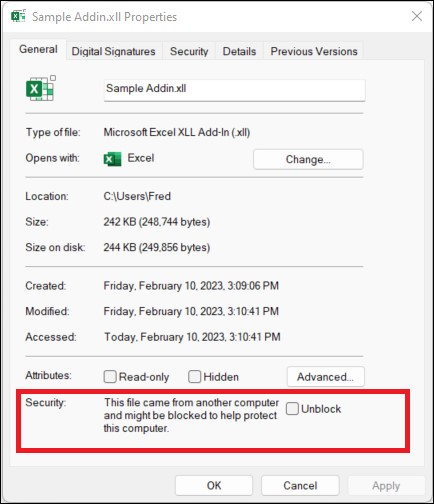
\includegraphics[width=0.35\textwidth]{file-properties-error.jpg}
    \caption{Windows MOTW Güvenlik Engeli ve Unblock (Engellemeyi Kaldır) Seçeneği}
    \label{fig:motw_unblock}
\end{figure}

\begin{itemize}
    \item[] \textbf{ActiveX Denetimleri ve Güvenlik Sınırlamaları:} Kod dinamik olarak \texttt{Forms.Frame.1}, \texttt{Forms.CommandButton.1} gibi OLE nesneleri oluşturur. Office güvenlik güncellemeleri veya Kill-Bit politikaları ActiveX denetimlerinin çalışma anında (\textit{runtime}) eklenmesini engelleyebilir. Excel Trust Center (Güven Merkezi) ayarlarından ActiveX denetimlerinin engellenmediğinden emin olunmalıdır.
\end{itemize}

% ==========================================
% AYRI SAYFA: KÜTÜPHANE VE EKSİK BİLEŞEN HATALARI
% ==========================================
\newpage

\paragraph{Kütüphane ve Eksik Bileşen (Reference) Hataları}
\vspace{0.2cm}

\begin{itemize}
    \item \textbf{Scripting.Dictionary (Windows Bağımlılığı):} Kod içerisinde \texttt{CreateObject \\ ("Scripting.Dictionary")} kullanılmıştır. macOS (Mac için Excel) üzerinde \texttt{scrrun.dll} bulunmadığı için kod \textit{Run-time error 429} hatası verir. Uygulama yalnızca Windows işletim sisteminde çalıştırılmalıdır.
    
    \vspace{0.3cm}
    
    \item \textbf{MSForms (Microsoft Forms 2.0 Object Library) Bağımlılığı:} Panel nesneleri \texttt{MSForms.Frame}, \texttt{MSForms.CommandButton} tipleriyle tanımlanmıştır. Excel kurulumunda VBA desteği eksikse veya nesne kütüphanelerinde bozulma (\textit{MISSING}) varsa "\textit{User-defined type not defined}" hatası alırsınız.
    
    Bu hatayı düzeltmek için klavyeden \textbf{\texttt{Alt + F11}} tuşlarına basarak VBA Editörüne girilmelidir. VBA penceresinde üst menüden \texttt{Tools -> References} seçeneğine tıklanmalı (Bkz. Şekil~\ref{fig:vba_references_all}) ve açılan listede \textit{Microsoft Forms 2.0 Object Library} kutucuğu işaretlenerek onaylanmalıdır.
\end{itemize}

\vspace{0.3cm}

% --- YAN YANA GÖRSELLER ---
\begin{figure}[htbp]
    \centering
    \begin{minipage}{0.45\textwidth}
        \centering
        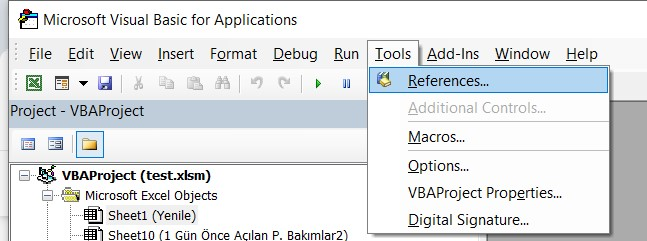
\includegraphics[width=\textwidth]{references1.jpg}
    \end{minipage}
    \hfill
    \begin{minipage}{0.45\textwidth}
        \centering
        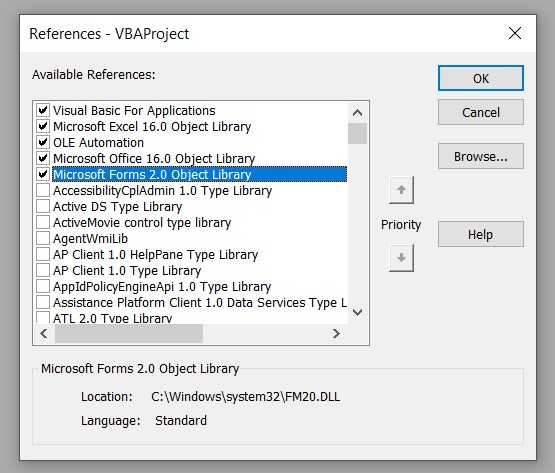
\includegraphics[width=\textwidth]{references2.jpg}
    \end{minipage}
    \caption{Alt + F11 ile VBA Editörüne Erişildikten Sonra Referans Ekleme Adımları (Solda: Tools -> References Menüsü, Sağda: MS Forms 2.0 Seçimi)}
    \label{fig:vba_references_all}
\end{figure}

\vspace{0.3cm}

\begin{itemize}
    \item \textbf{Arayüz Panellerinin Yüklenmemesi ve Manuel Yenileme:} Uygulama açılışında paneller temizlenip otomatik olarak yeniden inşa edildiği için (\texttt{Workbook\_Open} tetiklenmesiyle), ilk açılışta paneller görünmezse en pratik çözüm \textbf{dosyayı kaydedip kapatmak ve tekrar açmaktır}.
    
    Alternatif olarak; dosyayı kapatmadan panelleri yeniden yüklemek isterseniz, \textbf{"Yenile"} çalışma sayfasındayken klavyeden \textbf{\texttt{Alt + F8}} kısayol tuşlarına basabilir, açılan makro penceresinden \texttt{InitializeAppUI} fonksiyonunu seçerek \textbf{"Çalıştır"} (\textit{Run}) butonuna tıklayabilirsiniz.
\end{itemize}
\chapter{Uygulama Onarım Rehberi}

\section{Sayfa ve Panel Onarım Rehberi}

\begin{warningbox}
\textbf{\faExclamationTriangle\ Yenile Sayfası Kaybolduysa veya Silindiyse}

\vspace{0.2cm}
Sistem dinamik panel mimarisine sahiptir. Sayfa silindiğinde sıfırlama yapmadan önce kodların varlığını doğrulamak yeterlidir.

\textbf{Adım Adım Onarım Süreci:}
\begin{enumerate}\setlength{\itemsep}{1pt}
    \item \textbf{Kod Varlığını Doğrulayın:} \textbf{\texttt{Alt + F11}} ile VBA editörüne girip modüllerin (\texttt{mod\_*}) sol menüde yer aldığını teyit edin.
    \item \textbf{Yeni Sayfa Açın:} Excel arayüzünde \textbf{"Yenile"} adında yeni ve boş bir çalışma sayfası oluşturun.
    \item \textbf{Kaydedip Çıkın:} Dosyayı kaydedip kapatın. Yeniden açtığınızda otomasyon motoru yeni sayfayı algılayacak ve panelleri otomatik çizecektir.
\end{enumerate}
\end{warningbox}

\begin{infobox}
\textbf{\faDatabase\ ARIZA, BAKIM veya GECENAY Sayfaları Kaybolduysa}

\vspace{0.2cm}
Veritabanı sayfalarından biri silindiyse veya adı bozulduysa:
\begin{enumerate}\setlength{\itemsep}{1pt}
    \item Silinen sayfanın ismiyle (\texttt{ARIZA}, \texttt{BAKIM} veya \texttt{GECENAY}) birebir eşleşen yeni bir çalışma sayfası oluşturun.
    \item Takip eden sayfadaki \textbf{Ekran Görüntüsü Referanslarını} inceleyerek tablo ve sütun yapısını orijinal haline getirin.
    \item Sayfanın 1. satırına takip edilen tarihleri \texttt{dd.mm.yyyy} formatında ekleyin.
    \item Dosyayı kaydedip kapatın. Sistem bir sonraki açılışta veritabanı adreslerini bu sayfa üzerinden yeniden haritalayacaktır.
\end{enumerate}
\end{infobox}

\section{Tarih ve Dönem Yönetimi}

\begin{infobox}
\textbf{\faCalendar*\ Yeni Tarih Tanımlama Mantığı}

\vspace{0.2cm}
Sistem dinamik kesişim algoritması (\texttt{FindIntersectCell}) kullandığı için VBA kodlarında tarih güncellemesi yapmanıza gerek yoktur. \texttt{ARIZA} veya \texttt{BAKIM} sayfalarının 1. satırını yeni tarihlerle \texttt{dd.mm.yyyy} formatında değiştirmeniz yeterlidir.
\end{infobox}


% ==========================================
% 3 RESMİN TEK SAYFADA TOPLANDIĞI BÖLÜM
% ==========================================
\newpage
\section{Veritabanı Sayfa Yapıları ve Görsel Referanslar}

\begin{warningbox}
\textbf{\faExclamationCircle\ Sütun Doğruluğu, İsimler ve Hücre İçeriği Uyarısı}

\vspace{0.2cm}
Sayfalar yeniden oluşturulurken aşağıdaki kurallara \textbf{özellikle dikkat ediniz}:
\begin{itemize}\setlength{\itemsep}{1pt}
    \item Personel/Vaka \textbf{İsimlerinin B sütununda} (\texttt{B} kolonu) yazılması gerektiğini unutmayınız.
    \item \textbf{''AÇIK VAKA SAYISI''} ve \textbf{''KAPALI VAKA SAYISI''} başlıklarının bulunduğu sütunların harf doğruluğuna, hizalamasına ve hücre içeriklerine azami özen gösteriniz.
    \item Hatalı sütun veya isim yerleşimi arka plan servislerinin yanlış adreslere veri yazmasına veya kayıtları bulamamasına neden olur.
\end{itemize}
\end{warningbox}

\vspace{0.2cm}

\begin{figure}[htbp]
    \centering
    % 1. Resim: ARIZA
    \fboxsep=0pt
    \fboxrule=0.6pt
    \fcolorbox{bordergray}{white}{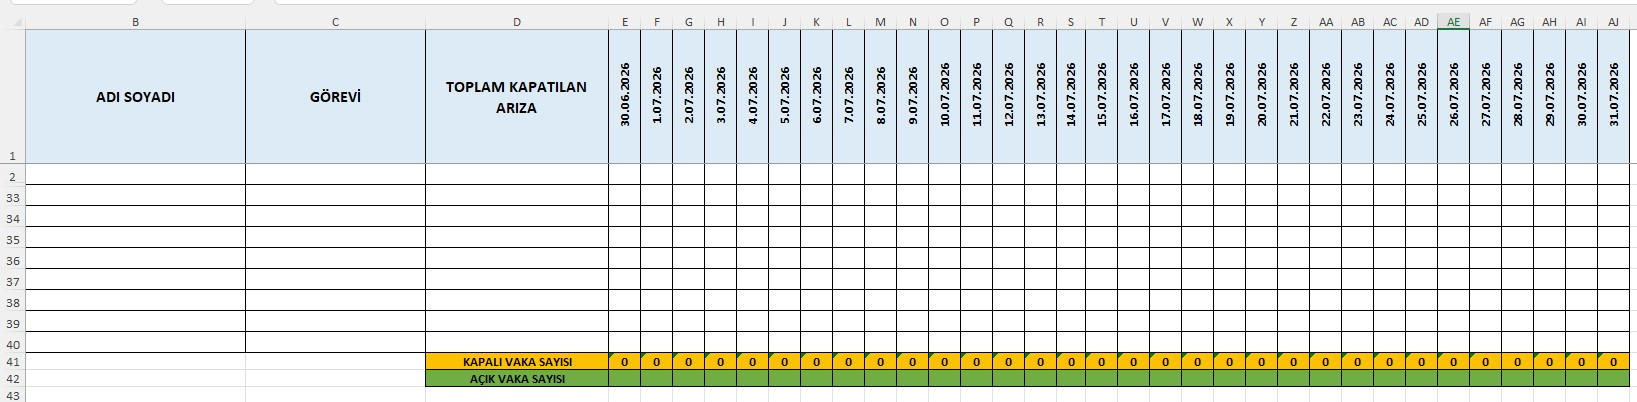
\includegraphics[width=0.92\textwidth, height=5.2cm, keepaspectratio]{ARIZA.jpg}}
    \caption*{ARIZA Sayfası Standart Tablo Yapısı (İsimler B Sütununda)}
    
    \vspace{0.2cm}
    
    % 2. Resim: BAKIM
    \fboxsep=0pt
    \fboxrule=0.6pt
    \fcolorbox{bordergray}{white}{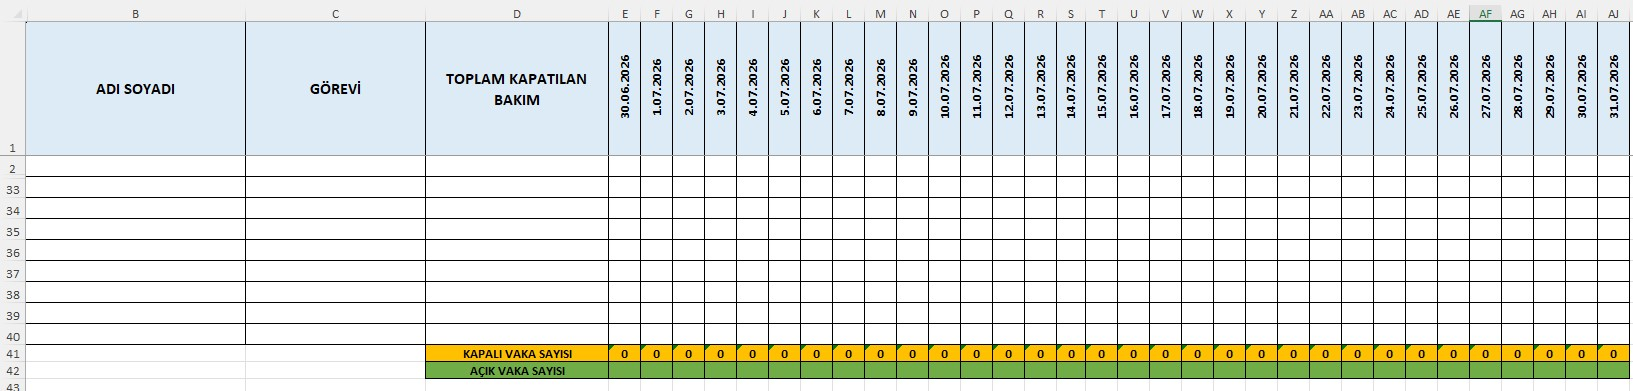
\includegraphics[width=0.92\textwidth, height=5.2cm, keepaspectratio]{BAKIM.jpg}}
    \caption*{BAKIM Sayfası Standart Tablo Yapısı (İsimler B Sütununda)}
    
    \vspace{0.2cm}
    
    % 3. Resim: GECENAY
    \fboxsep=0pt
    \fboxrule=0.6pt
    \fcolorbox{bordergray}{white}{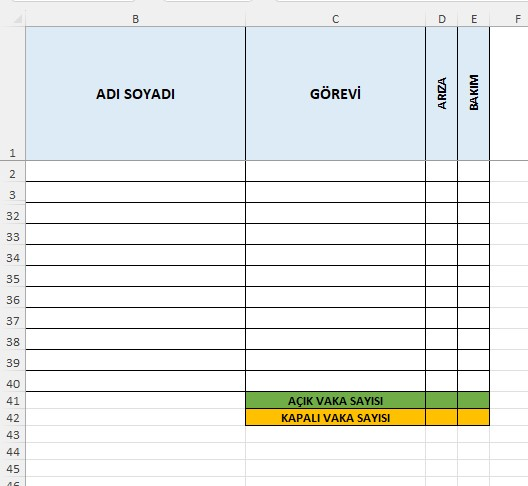
\includegraphics[width=0.92\textwidth, height=5.2cm, keepaspectratio]{GECENAY.jpg}}
    \caption*{GECENAY Sayfası Standart Tablo Yapısı (İsimler B Sütununda)}
    
    \caption{Veritabanı Sayfaları Standart Tablo Düzenleri (ARIZA, BAKIM, GECENAY)}
    \label{fig:all_db_sheets}
\end{figure}
\chapter{Proje Dosya Yapısı ve Mimari}

\noindent
% -------------------------------------------------------------------------
% SOL KOLON (Görsel ve Sheet Mantığı)
% -------------------------------------------------------------------------
\begin{minipage}[t]{0.48\textwidth}
    {\Large \bfseries \textcolor{primary}{VBA Proje Ağacı}} \\[0.15cm]
    \small Projede yer alan tüm dosya, modül ve sınıf yapıları katmanlı mimari (\textit{Layered Architecture}) prensiplerine uygun kurgulanmıştır.

    \vspace{0.25cm}

    % Proje Ağacı Görseli
    \centering
    \fboxsep=0pt
    \fboxrule=0.5pt
    \fcolorbox{bordergray}{white}{%
        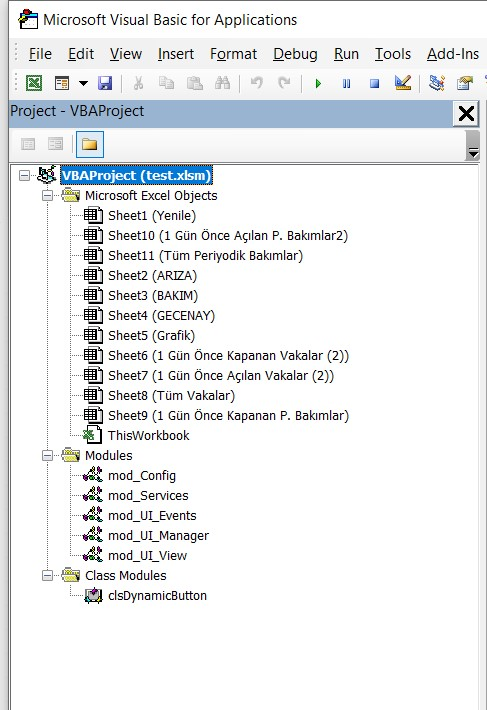
\includegraphics[width=0.90\linewidth, height=7.5cm, keepaspectratio]{project_files.jpg}%
    }
    \captionof{figure}{VBA Proje Ağacı}

    \vspace{0.3cm}

    \begin{tcolorbox}[colback=lightgray,colframe=bordergray,leftrule=3.5pt,boxrule=0.4pt,top=4.5pt,bottom=4.5pt]
        \textbf{\textcolor{primary}{\faFileExcel\ Excel Sheet Modülleri:}}\\
        \small Projede yer alan \textbf{Sheet1 (Yenile)}, \textbf{Sheet2 (ARIZA)}, \textbf{Sheet3 (BAKIM)} ve \textbf{Sheet4 (GECENAY)} gibi yerleşik sayfaların içerisine kod yazılmamıştır. 

        Kolay okunur kod yapısı sağlamak amacıyla tüm olaylar servis katmanına yönlendirilmiştir.
    \end{tcolorbox}
    
    \vspace{0.15cm}

    \begin{tcolorbox}[colback=lightgray,colframe=bordergray,leftrule=3.5pt,boxrule=0.4pt,top=4.5pt,bottom=4.5pt]
        \textbf{\textcolor{primary}{\faBook\ ThisWorkbook:}}\\
        \small Çalışma kitabı açılış/kapanış olaylarını (\texttt{Workbook\_Open}) ve sistem ilklendirme süreçlerini yönetir.
    \end{tcolorbox}
\end{minipage}
\hfill
% -------------------------------------------------------------------------
% SAĞ KOLON (Modüller ve Class)
% -------------------------------------------------------------------------
\begin{minipage}[t]{0.48\textwidth}
    {\Large \bfseries \textcolor{primary}{Standart Modüller}} \\[0.2cm]

    \begin{tcolorbox}[colback=lightgray,colframe=bordergray,leftrule=3pt,boxrule=0.4pt,top=4.5pt,bottom=4.5pt]
        \textbf{\textcolor{primary}{\faCog\ mod\_Config:}}\\
        \small Sabitler (Constants), renk kodları, hücre adresi eşleşmeleri ve konfigürasyon değişkenlerini barındırır.
    \end{tcolorbox}

    \begin{tcolorbox}[colback=lightgray,colframe=bordergray,leftrule=3pt,boxrule=0.4pt,top=4.5pt,bottom=4.5pt]
        \textbf{\textcolor{primary}{\faServer\ mod\_Services:}}\\
        \small Veri arama, tarih doğrulamaları ve arka plan hesaplamalarını yürüten ana iş mantığı (Business Logic) katmanıdır.
    \end{tcolorbox}

    \begin{tcolorbox}[colback=lightgray,colframe=bordergray,leftrule=3pt,boxrule=0.4pt,top=4.5pt,bottom=4.5pt]
        \textbf{\textcolor{primary}{\faMousePointer\ mod\_UI\_Events:}}\\
        \small Kullanıcı etkileşimleri ve sayfa içi olay yönlendirmelerini dinleyen event modülüdür.
    \end{tcolorbox}

    \begin{tcolorbox}[colback=lightgray,colframe=bordergray,leftrule=3pt,boxrule=0.4pt,top=4.5pt,bottom=4.5pt]
        \textbf{\textcolor{primary}{\faSlidersH\ mod\_UI\_Manager:}}\\
        \small Arayüz elemanlarının koordinasyonu ve oturum durumlarının yönetildiği katmandır.
    \end{tcolorbox}

    \begin{tcolorbox}[colback=lightgray,colframe=bordergray,leftrule=3pt,boxrule=0.4pt,top=4.5pt,bottom=4.5pt]
        \textbf{\textcolor{primary}{\faPaintBrush\ mod\_UI\_View:}}\\
        \small Dinamik panellerin çizimi ve görsel bileşenlerin sayfaya basılmasından sorumlu arayüz katmanıdır.
    \end{tcolorbox}

    \vspace{0.4cm}

    {\Large \bfseries \textcolor{primary}{Sınıf Modülleri}} \\[0.2cm]

    \begin{tcolorbox}[colback=lightgray,colframe=bordergray,leftrule=3.5pt,boxrule=0.4pt,top=4.5pt,bottom=4.5pt]
        \textbf{\textcolor{primary}{\faCube\ clsDynamicButton:}}\\
        \small Sayfa üzerinde çalışma zamanında (runtime) dinamik olarak oluşturulan butonların tıklanma olaylarını (Event-Handling) nesne tabanlı olarak yöneten sınıf yapısıdır.
    \end{tcolorbox}
\end{minipage}
\chapter{VBA Nedir ve Temel Kavramlar}


% ==========================================
% SAYFA 1: GİRİŞ VE MİMARİNİN TEMEL BİLEŞENLERİ
% ==========================================

\section{VBA (Visual Basic for Applications) Nedir?}

VBA, Microsoft Office uygulamalarının arka planında çalışan, iş akışlarını otomatikleştirmek ve özel iş mantıkları (Business Logic) yürütmek için kullanılan nesne yönelimli ve olay güdümlü bir programlama dilidir. Excel başta olmak üzere Word, Outlook, Access gibi tüm Office araçlarında yerleşik olarak bulunur.

\begin{infobox}{\faTerminal\ Projedeki Temel Rolü}
Bu projede VBA; hücre bazlı manuel işlemleri ortadan kaldırarak arka planda çalışan servis fonksiyonları üzerinden vaka tarama, tarih matrisi eşleştirme ve veritabanı kayıt süreçlerini otomatikleştirir.
\end{infobox}

\vspace{0.1cm}

\section{Excel VBA Temel Bileşenleri}

Bir Excel projesindeki VBA bileşenleri varsayılan (yerleşik) ve geliştirici tarafından eklenen özel yapılar olarak ikiye ayrılır. Projede kullanılan mimari bileşenler ve varlık durumları aşağıda özetlenmiştir:

\begin{table}[h!]
\centering
\small
\begin{tabular}{p{0.22\linewidth} p{0.25\linewidth} p{0.46\linewidth}}
\toprule
\textbf{Bileşen Türü} & \textbf{Varlık Durumu} & \textbf{Sistemdeki Görevi ve Kullanım Amacı} \\
\midrule
\textbf{ThisWorkbook} & Yerleşik \textit{(Her Projede var)} & Dosya açılış/kapanış olaylarını dinler.\\
\textbf{Sheet Modülleri} & Yerleşik \textit{(Her Projede var)} & Sayfaya özel olayları dinler. \textit{(Bu projede temiz mimari için boş bırakılmıştır)} \\
\textbf{Standart Modül} & Özel \textit{(Eklenir - \texttt{.bas})} & Arka plan servis fonksiyonlarını ve genel hesaplama mantıklarını barındırır. \\
\textbf{Sınıf Modülü} & Özel \textit{(Eklenir - \texttt{.cls})} & Nesne tabanlı programlama (OOP) sağlar. \\
\textbf{UserForm} & Özel \textit{(Eklenir - \texttt{.frm})} & Form arayüzüdür. \textit{(Bu projede UI karmaşıklığını önlemek için kullanılmamıştır)}. \\
\bottomrule
\end{tabular}
\caption{VBA Bileşenlerinin Projedeki ve Excel'deki Yapısal Durumu}
\end{table}

\begin{warningbox}{\faExclamationCircle\ Proje Mimarisi Notu}
Bu projede kullanıcı arayüzü karmaşıklığını önlemek adına \textbf{UserForm kullanılmamış} ve kod bağımlılığını azaltmak için \textbf{Sheet modüllerine kod yazılmamıştır}. Tüm otomasyon mantığı Standart ve Class modülleri üzerinden servis odaklı yürütülmektedir.
\end{warningbox}

\newpage

% ==========================================
% SAYFA 2: PROGRAMLAMA MANTIĞI VE TEMEL DİL YAPILARI
% ==========================================

\section{VBA Programlama Mantığı ve Temel Yapılar}

VBA (Visual Basic for Applications), nesne tabanlı ve olay güdümlü mimarisiyle performanslı otomasyonlar oluşturulmasını sağlar. Profesyonel VBA geliştirmede bellek yönetimi, değişken bildirimleri ve modüler kod tasarımı temel yapı taşlarıdır.

\begin{tcolorbox}[colback=lightgray,colframe=bordergray,leftrule=3.5pt,boxrule=0.4pt,top=5pt,bottom=5pt]
    \textbf{\textcolor{primary}{\faShield*\ Katı Değişken Tanımlama (\texttt{Option Explicit}):}}
    Modülün en başında yer alan \texttt{Option Explicit} bildirimi, değişkenlerin önceden tanımlanmasını (\texttt{Dim}) zorunlu kılar. Bu standart; yazım hatalarından doğan mantıksal hataları (bug) engeller, yanlış veri türü kullanımının önüne geçer ve bellekte gereksiz alan tahsisini önleyerek çalışma zamanı performansını optimize eder.
\end{tcolorbox}

\begin{tcolorbox}[colback=lightgray,colframe=bordergray,leftrule=3.5pt,boxrule=0.4pt,top=5pt,bottom=5pt]
    \textbf{\textcolor{primary}{\faCube\ Nesne Hiyerarşisi (DOM) ve Bellek Yönetimi:}}
    VBA hiyerarşik bir nesne modeli kullanır (\texttt{Application} $\rightarrow$ \texttt{Workbook} $\rightarrow$ \texttt{Worksheet} $\rightarrow$ \texttt{Range}). Kod içerisinde hücre veya sayfa işlemleri yapılırken nesnelerin bir değişkene atanarak (\texttt{Set ws = ThisWorkbook.Sheets(...)}) başvurulması, Excel'in grafik arayüz yükünü azaltır ve çalışma süresini ciddi oranda kısaltır.
\end{tcolorbox}

\begin{tcolorbox}[colback=lightgray,colframe=bordergray,leftrule=3.5pt,boxrule=0.4pt,top=5pt,bottom=5pt]
    \textbf{\textcolor{primary}{\faCodeBranch\ Prosedür (Sub) ve Fonksiyon (Function) Mimarisi:}}
    VBA'de kod blokları işlevlerine göre iki ana yapıya ayrılır:
    \begin{itemize}
        \item \textbf{Sub (Prosedür):} Belirli bir eylem dizisini çalıştırır ancak geriye bir değer döndürmez. Genellikle buton tetiklemeleri, arayüz ilklendirmeleri ve akış kontrolü için kullanılır (Örn: \texttt{InitializeAppUI}).
        \item \textbf{Function (Fonksiyon):} Parametre alıp veri işleyen ve işlem sonucunda geriye bir değer döndüren yapılardır. Hesaplama, arama ve veri doğrulama işlemleri için tercih edilir (Örn: \texttt{GetReportDate}).
    \end{itemize}
\end{tcolorbox}

\begin{tcolorbox}[colback=lightgray,colframe=bordergray,leftrule=3.5pt,boxrule=0.4pt,top=5pt,bottom=5pt]
    \textbf{\textcolor{primary}{\faDatabase\ Veri Tipleri ve Değişken Seçim Mantığı:}}
    VBA'de performans doğrudan seçilen veri tiplerine bağlıdır. Tam sayılar için \texttt{Long} (16-bit Integer yerine 32-bit bellek optimizasyonu), metinler için \texttt{String}, mantıksal değerler için \texttt{Boolean} ve esnek/bilinmeyen veriler için \texttt{Variant} kullanılır. Yanlış veri tipi seçimi bellek şişmesine veya işlem yavaşlığına yol açar.
\end{tcolorbox}

\vspace{0.1cm}

\begin{warningbox}{\faExclamationTriangle\ Hata Yönetimi ve İstisna Kontrolü (Error Handling)}
VBA'de beklenmeyen hataların uygulamayı çökertmesini önlemek için \texttt{On Error} mekanizmaları kullanılır. Riskli işlemlerden önce \texttt{On Error Resume Next} ile istisnalar es geçilip kontrol edilebilir; işlem tamamlandığında ise sistemin varsayılan hata yakalama moduna dönmesi için hemen \texttt{On Error GoTo 0} ifadesi çalıştırılmalıdır.
\end{warningbox}

\vspace{0.1cm}

\begin{warningbox}{\faTachometer*\ Ekran Yenileme ve Performans Optimizasyonu}
Büyük veri kümeleriyle çalışırken ekranın her işlemde güncellenmesini engellemek için kod başında \texttt{Application.ScreenUpdating = False} ve otomatik hesaplamaları durdurmak için \texttt{Application.Calculation = xlCalculationManual} komutları kullanılır. İşlem bitiminde bu ayarların tekrar aktif edilmesi kritik önem taşır.
\end{warningbox}



\newpage

% ==========================================
% SAYFA 3: ÖRNEK KOD BLOĞU VE DETAYLI İNCELEME
% ==========================================

\section{Projeden Örnek Kod Bloğu ve İncelemesi}

Aşağıdaki kod parçacığı, projenin servis katmanından (\texttt{mod\_Services}) alınmış gerçek bir fonksiyondur. Fonksiyon, kendisine verilen herhangi bir Excel sayfasının ilk satırını tarayarak geçerli rapor tarihini tespit eder:

\begin{lstlisting}[caption={Rapor Tarihi Tespit Servis Fonksiyonu (mod\_Services)}]
' Retrieves the report date from the specified worksheet header row.
Public Function GetReportDate(ws As Worksheet) As String
    Dim col As Long, cellVal As Variant
    GetReportDate = STATUS_NOT_FOUND
    For col = 1 To 50
        cellVal = ws.Cells(1, col).Value
        If Not IsEmpty(cellVal) And IsDate(cellVal) Then
            GetReportDate = Format(CDate(cellVal), "dd.mm.yyyy")
            Exit Function
        End If
    Next col
End Function
\end{lstlisting}

\vspace{0.2cm}
\noindent \textbf{Kodun Çalışma Mantığı ve Adım Adım Analizi}\\

Yukarıdaki kod bloğu, modüler bir VBA servis fonksiyonunun tüm standartlarını içermektedir:

\begin{enumerate}
    \item \textbf{Girdi ve Çıktı Tanımı:} \texttt{Public Function GetReportDate(ws As Worksheet) As String} satırı ile fonksiyon dışarıdan bir Excel sayfası nesnesi (\texttt{ws}) alır ve işlem sonucunda metinsel (\texttt{String}) bir tarih değeri döndürür.
    \item \textbf{Değişken Deklarasyonu:} Döngü sayacı için \texttt{col As Long} ve hücre içeriğini tutmak için esnek veri tipi olan \texttt{cellVal As Variant} tanımlanmıştır.
    \item \textbf{Varsayılan Durum (Fallback):} \texttt{GetReportDate = STATUS\_NOT\_FOUND} ifadesiyle, taramada tarih bulunamazsa fonksiyonun çökmeden güvenli bir durum döndürmesi sağlanır.
    \item \textbf{Döngü Yönetimi ve Doğrulama:} \texttt{For col = 1 To 50} komutu ile ilk satırın 1. sütunundan 50. sütununa kadar olan hücreler taranır. \texttt{If Not IsEmpty(cellVal) And IsDate(cellVal)} koşuluyla hücrenin dolu ve geçerli bir tarih olduğu teyit edilir.
    \item \textbf{Biçimlendirme ve Erken Çıkış:} Tarih bulunduğunda \texttt{Format(..., "dd.mm.yyyy")} ile standart biçime çevrilir ve \texttt{Exit Function} komutuyla kalan sütunlar taranmadan işlem anında bitirilir.
\end{enumerate}

\vspace{0.2cm}

\begin{infobox}{\faSitemap\ Genel Çalışma Mimarisi ve Modülerliğin Avantajı}
Kullanıcı arayüzünde (UI katmanı) yer alan dinamik ListBox, Form ve Buton gibi tüm bileşenler verileri doğrudan hücrelerden okumak yerine bu \textbf{Servis Modüllerini (\texttt{mod\_Services})} çalıştırır. 

Bu modüler yaklaşım sayesinde:
\begin{itemize}
    \item İş mantığı (Business Logic) ile Görsel Arayüz (UI) birbirinden tamamen ayrılır.
    \item Sayfa yapısı veya Excel tasarımı değişse bile sadece servis fonksiyonu güncellenir; arayüz kodlarına dokunmak gerekmez.
    \item Aynı hesaplama ve tarama fonksiyonu projenin farklı yerlerinde tekrar tekrar güvenle kullanılabilir (Reusability).
\end{itemize}
\end{infobox}
\chapter{Detaylı Modül İncelemeleri}

% ==========================================
% BÖLÜM 4.1: THISWORKBOOK (ÇALIŞMA KİTABI ETKİLEŞİM KATMANI)
% ==========================================

\section{\texttt{ThisWorkbook}}

\texttt{ThisWorkbook}, Excel VBA mimarisinde çalışma kitabının yaşam döngüsünü (\textit{Lifecycle}) ve global olayları (\textit{Workbook-Level Events}) dinleyen yerleşik sınıf modülüdür. Projede uygulamanın otomatik ilklendirilmesini (\textit{Initialization}) ve bellek değişkenlerinin hazırlanmasını sağlar.

Excel açıldığında grafik motoru, OLE bileşenleri ve Active Document yapısı henüz yüklenmemiş olabilir. Bu süreçte doğrudan makro çalıştırmak veya arayüze OLE nesneleri çizmek; grafik kaymalarına ve Korumalı Görünüm (\textit{Protected View}) modunda uygulamanın aniden çökmesine neden olur.

\texttt{ThisWorkbook} modülü, söz konusu kararsızlığı önlemek adına **Asenkron Gecikmeli Başlatma (Asynchronous Delayed Execution)** mimari desenini uygular:

\begin{itemize}\setlength{\itemsep}{0pt}\setlength{\parskip}{1pt}
    \item \textbf{Yerleşik Olay Yakalama (\texttt{Workbook\_Open}):} Otomatik tetiklenen giriş noktasıdır (\textit{Entry Point}).
    \item \textbf{İşlem Oluğu Sıfırlama (\texttt{DoEvents}):} Bekleyen tüm grafik yenileme ve ekran çizim olaylarını zorunlu kılar.
    \item \textbf{Zamanlanmış Tetikleme (\texttt{Application.OnTime}):} Arayüz kurma fonksiyonu olan \texttt{InitializeAppUI} prosedürünü 1 saniyelik mikro gecikmeyle Excel yürütme kuyruğuna kaydeder.
\end{itemize}

\vspace{0.15cm}

\begin{infobox}{\faClock\ Asenkron Başlatmanın Sistem Performansına Etkisi}
\texttt{Application.OnTime Now + TimeValue("00:00:01"), "InitializeAppUI"} kullanımı, dosya açılışında Excel UI motorunun tamamen stabil hale gelmesini bekler. Bu sayede servisler ve dinamik butonlar çökme riski olmadan sıfır hatayla ilklendirilir.
\end{infobox}

\vspace{0.15cm}

Aşağıdaki kod bloğu, projedeki \texttt{ThisWorkbook} sınıf modülünün tam yapısını içermektedir:

\begin{lstlisting}[caption={ThisWorkbook Sınıf Modülü Kod Yapısı}]
'*****************************************************************************
' Class: ThisWorkbook
' Purpose: Standard class module that handles workbook-level events.
'*****************************************************************************

Private Sub Workbook_Open()
    DoEvents
    Application.OnTime Now + TimeValue("00:00:01"), "InitializeAppUI"
End Sub
\end{lstlisting}

\newpage

% ==========================================
% BÖLÜM 4.2: CLSDYNAMICBUTTON (DİNAMİK NESNE TABANLI OLAY KONTROLÜ)
% ==========================================

\section{\texttt{clsDynamicButton}}

\texttt{clsDynamicButton}, çalışma zamanında (\textit{Runtime}) üretilen butonların tıklanma olaylarını (\texttt{Click Event}) Nesne Tabanlı Programlama (OOP) prensipleri doğrultusunda dinamik olarak yakalayan özel bir Sınıf Modülüdür (\textit{Class Module}).

UserForm kullanılmayan mimarilerde arayüz elemanları doğrudan \texttt{Worksheet} üzerine çizilir. Ancak dinamik eklenen bir \texttt{MSForms.CommandButton} nesnesinin statik bir tıklama prosedürü bulunmaz. Bu kısıtlamayı aşmak adına projedeki her bir dinamik buton, \texttt{clsDynamicButton} sınıfından türetilen bir nesneye bağlanır ve bellek ömrünü uzatmak için global bir koleksiyonda saklanır.

Sınıf içerisindeki \texttt{WithEvents} bildirimi, buton etkileşimlerini anlık dinler. Tıklama anında izlenen işlem adımları:

\begin{itemize}\setlength{\itemsep}{0pt}\setlength{\parskip}{1pt}
    \item \textbf{Referans ve Kapsayıcı Tespiti:} Tıklanan buton örneği yakalanır ve üst paneli (\texttt{MSForms.Frame}) doğrulanır.
    \item \textbf{Olay Delegasyonu:} Panelin adına göre (\texttt{pan\_Login}, \texttt{pan\_OSM} vb.) tetiklenecek yönlendirme \texttt{mod\_UI\_Events} modülündeki handler fonksiyonlarına aktarılır.
\end{itemize}

\vspace{0.15cm}

\begin{warningbox}{\faExclamationTriangle\ Bellek Yönetimi ve Nesne Yaşam Ömrü (Garbage Collection)}
VBA bellek yöneticisi, referansı tutulmayan sınıf örneklerini anında siler. Dinamik butonların tıklama olaylarının aktif kalması için \texttt{clsDynamicButton} örneklerinin \texttt{ButtonCollection} koleksiyonuna \texttt{Add} metoduyla eklenmesi kritik önem taşır.
\end{warningbox}

\vspace{0.15cm}

Aşağıdaki kod bloğu, dinamik buton olaylarını dinleyen ve ilgili UI panellerine yönlendiren sınıf yapısını özetlemektedir:

\begin{lstlisting}[caption={clsDynamicButton Sınıf Modülü Kod Yapısı}]
'*****************************************************************************
' Class: clsDynamicButton
' Purpose: This class is used to handle events for dynamically created buttons.
'*****************************************************************************

Public WithEvents DynamicButton As MSForms.CommandButton

Private Sub DynamicButton_Click()
    Dim parentFrame As MSForms.Frame
    
    On Error Resume Next
    Set parentFrame = DynamicButton.Parent
    On Error GoTo 0

    If parentFrame Is Nothing Then Exit Sub

    Select Case parentFrame.Name
        Case "pan_Login":    mod_UI_Events.HandleLoginPanelEvents DynamicButton.Name, parentFrame
        Case "pan_OSM":      mod_UI_Events.HandleOSMPanelEvents DynamicButton.Name, parentFrame
        Case "pan_Open":     mod_UI_Events.HandleOpenPanelEvents DynamicButton.Name, parentFrame
        ' . . . (pan_Closed, pan_PreviousMonth, pan_SelectPreviousMonth, ....)
    End Select
End Sub
\end{lstlisting}


% ==========================================
% BÖLÜM 4.3: MOD_CONFIG (GLOBAL YAPILANDIRMA VE SABİTLER)
% ==========================================

\section{\texttt{mod\_Config}}

\texttt{mod\_Config}, uygulamanın tüm merkezi sabitlerini, metinsel ifadelerini, renk paletini ve veritabanı sütun eşlemelerini bünyesinde barındıran standart kod modülüdür (\textit{Standard Module}). Kod karmaşıklığını önlemek ve bakımı kolaylaştırmak adına proje içerisindeki hiçbir fonksiyona sert kodlanmış (\textit{Hardcoded}) metin veya sayısal değer yazılmamıştır.

Gelecekte projede yapılabilecek güncellemeler doğrudan bu modül üzerinden yönetilir:

\begin{itemize}\setlength{\itemsep}{0pt}\setlength{\parskip}{1pt}
    \item \textbf{Arayüz Metinleri ve Açılır Pencereler (Pop-up):} Arayüzdeki buton yazıları (\texttt{BTN\_CAPTION}), panel başlıkları (\texttt{LBL\_TITLE}) veya kullanıcıya gösterilen tüm uyarı/bilgi bildirim mesajları (\texttt{MSG\_*}) değiştirilmek istendiğinde yalnızca bu modüldeki ilgili sabitler güncellenir.
    \item \textbf{Veritabanı ve Sütun Yapısı Değişiklikleri:} İlerleyen süreçte \texttt{ARIZA}, \texttt{BAKIM} veya \texttt{GECENAY} sayfalarında sütun yerleri veya aranan metin bağlamları değişirse; \texttt{DB\_*}, \texttt{CLOSED\_*} ve \texttt{PREV\_MONTH\_*} grubu altında tanımlanan sütun harfleri (\texttt{"A"}, \texttt{"D"}, \texttt{"K"} vb.) kolayca revize edilebilir.
\end{itemize}

\vspace{0.15cm}

\begin{infobox}{\faCogs\ Merkezi Yönetim ve Bakım Kolaylığı}
Uygulamanın renk paleti (\texttt{COLOR\_GREEN}, \texttt{COLOR\_RED}), panel boyutları (\texttt{PANEL\_WIDTH}) ve dinamik buton referanslarını tutan global \texttt{ButtonCollection} koleksiyonu bu modülde tanımlanarak projenin modülerliği garanti altına alınmıştır.
\end{infobox}

\vspace{0.15cm}

Aşağıdaki kod bloğu, \texttt{mod\_Config} modülünün kategorize edilmiş temsilî yapısını göstermektedir:

\begin{lstlisting}[caption={mod\_Config Modülü Sabit ve Yapılandırma Tanımları}]
'*****************************************************************************
' Module: mod_Config
' Purpose: Global configuration settings, constants, and variables.
'*****************************************************************************

' 1. SAYFA VE VERİTABANI İSİMLERİ (ARIZA, BAKIM, GECENAY)
Public Const MAIN_SHEET_NAME           As String = "Yenile"
Public Const PREVIOUS_MONTH_SHEET_NAME As String = "GECENAY"
Public Const DATABASE_SHEET_NAME_ARIZA As String = "ARIZA"
Public Const DATABASE_SHEET_NAME_BAKIM As String = "BAKIM"

' 2. VERİTABANI SÜTUN EŞLEMELERİ (COLUMN MAP)
Public Const DB_OSM_DATES_START_COL As String = "A"
Public Const DB_OPEN_CELL_COL       As String = "D"
Public Const DB_CLOSED_NAME_COL     As String = "B"
Public Const ALL_CASES_ASSIGNED_COL As String = "K"
' . . . (Diğer sütun ve hücre adres tanımlamaları)

' 3. POP-UP BİLDİRİM VE UYARI MESAJLARI (MESSAGES)
Public Const MSG_OPEN_SAVE_SUCCESS   As String = "Açık kayıt sayıları veritabanına kaydedildi."
Public Const MSG_ALL_OPERATIONS_COMPLETED As String = "Tüm güncelleme işlemleri başarıyla tamamlandı!"
' . . . (Diğer bildirim ve hata mesajları)

' 4. GLOBAL DEĞİŞKENLER VE ETKİLEŞİM KOLEKSİYONU
Public ButtonCollection As New Collection
\end{lstlisting}


\newpage

% ==========================================
% BÖLÜM 4.4: MOD_UI_MANAGER (PANEL VE ARAYÜZ YÖNETİMİ)
% ==========================================

\section{\texttt{mod\_UI\_Manager}}

\texttt{mod\_UI\_Manager}, dinamik panel geçişlerini, OLE nesnelerinin bellek yönetimini ve oturum kilit durumlarını orkestre eden servis katmanıdır. Sayfa üzerindeki tüm arayüz döngüsünün orkestrasyonunu üstlenir.

\vspace{0.3cm}

\textbf{\textcolor{primary}{1. \texttt{InitializeAppUI} Prosedürü}}

Çalışma kitabı açıldığında veya oturum sıfırlandığında tetiklenen ilk ilklendirme giriş noktasıdır. Uygulama altyapısını sırayla ayağa kaldırır.

\begin{lstlisting}[caption={InitializeAppUI Prosedürü Kod Yapısı}]
Public Sub InitializeAppUI()
    If Not Application.ActiveProtectedViewWindow Is Nothing Then Exit Sub
    Dim ws As Worksheet
    On Error Resume Next
    Set ws = ThisWorkbook.Sheets(MAIN_SHEET_NAME)
    On Error GoTo 0
    If ws Is Nothing Then Exit Sub
    
    BuildNavigationSystem
    SwitchTo "Login"
    
    With ws
        .ScrollArea = "A1"
        .EnableSelection = xlNoSelection
    End With
End Sub
\end{lstlisting}

\begin{infobox}{\faPlay\ Fonksiyon Özeti}
Navigasyon altyapısını kurup açılış ekranı olarak \texttt{Login} panelini çağırır. Kullanıcının sayfa hücreleriyle doğrudan etkileşime girmesini engellemek adına \texttt{ScrollArea} ve seçim izinlerini kısıtlar.
\end{infobox}

\vspace{0.3cm}

\textbf{\textcolor{primary}{2. \texttt{BuildNavigationSystem} Prosedürü}}

Tüm arayüz panellerini sıfırdan oluşturan ve bellek üzerindeki eski nesne referanslarını güvenle temizleyen yapıcı kısımdır.

\begin{lstlisting}[caption={BuildNavigationSystem Prosedürü (Özet)}]
Public Sub BuildNavigationSystem()
    ' Dynamic Button Koleksiyonunu ve OLE Nesnelerini Temizleme
    If Not ButtonCollection Is Nothing Then
        Dim btnItem As Object
        For Each btnItem In ButtonCollection
            Set btnItem.DynamicButton = Nothing
        Next btnItem
        Set ButtonCollection = Nothing
    End If
    Set ButtonCollection = New Collection
    
    ' . . . (bx_Anchor kontrolü ve eski OLE nesnelerinin temizlenmesi)
    
    ' Panellerin mod_UI_View Üzerinden Çizilmesi
    mod_UI_View.CreateLoginPanel ws
    mod_UI_View.CreateOSMPanel ws
    mod_UI_View.CreateOpenPanel ws
    ' . . . (Closed, PreviousMonth vb. diğer panellerin oluşturulması)
End Sub
\end{lstlisting}

\newpage

\textbf{\textcolor{primary}{3. \texttt{SwitchTo} Prosedürü}}

Paneller arası görünürlük geçişini ve liste bileşenlerinin dinamik veriye bağlanmasını sağlayan ana yönlendirme fonksiyonudur.

\begin{lstlisting}[caption={SwitchTo Prosedürü (Özet)}]
Public Sub SwitchTo(panelName As String)
    Dim ws As Worksheet, oleObj As OLEObject, realFrame As MSForms.Frame
    Set ws = ThisWorkbook.Sheets(MAIN_SHEET_NAME)
    If ws.OLEObjects("pan_" & panelName) Is Nothing Then Exit Sub
    
    ' Tüm Panelleri Gizle ve Hedef Paneli Konumlandır
    ' . . . (ws.OLEObjects("pan_*").Visible = False ve hedef panel hizalama)

    Set realFrame = oleObj.Object
    
    ' Panele Özel ListBox Formatlaması ve Render Yönlendirmesi
    Select Case panelName
        Case "OSM"
            ' . . . (lst_Status genişlik/sütun ayarları)
            mod_UI_View.RenderOSMSheetStatus realFrame, False
        Case "Open"
            ' . . . (lst_OpenStatus genişlik/sütun ayarları)
            mod_UI_View.RenderOpenSheets realFrame
        ' . . . (Closed, PreviousMonth vb. diğer Case yapıları)
    End Select
End Sub
\end{lstlisting}

\begin{infobox}{\faCog\ Fonksiyon Özeti}
Diğer servis ve event modüllerinden tek satırla çağrılarak yumuşak panel geçişi sağlar. Ekrandaki tüm panelleri gizleyip hedef paneli hizalar, \texttt{ListBox} sütun ayarlarını yapar ve ilgili \texttt{Render} prosedürünü tetikler.
\end{infobox}

\vspace{0.3cm}

\textbf{\textcolor{primary}{4. Yardımcı Kilit Fonksiyonları (\texttt{LockPanel} vb.)}}

İş akışı sırasında geçersiz durumlarda kullanıcının hatalı adım atmasını önlemek amacıyla buton erişimlerini kısıtlayan yardımcı prosedürlerdir.

\begin{infobox}{\faLock\ Fonksiyon Özeti}
\texttt{LockPanel} ve \texttt{LockPreviousMonthPanel} prosedürleri; işlem adımları tamamlandığında ilgili panellerdeki "Sonraki Adım" butonlarının \texttt{Enabled} özelliğini \texttt{False} konumuna getirip renklerini griye dönüştürerek geçişleri kilitler.
\end{infobox}

\vspace{0.4cm}


\begin{tcolorbox}[colback=yellow!15,colframe=orange!80!black,leftrule=3.5pt,boxrule=0.4pt,top=6pt,bottom=6pt]
    \textbf{\textcolor{orange!80!black}{\faInfoCircle\ mod\_UI\_Manager Genel Özet ve Mimari Rolü:}}\\
    \small \texttt{mod\_UI\_Manager}, arayüzün dinamik yaşam döngüsünü tamamen arka plandaki iş mantığından (\textit{Business Logic}) ve çizim bileşenlerinden (\textit{View Layer}) soyutlar. 
    
    Tüm panel oluşturma, temizleme, boyutlandırma ve erişim kısıtlama süreçlerini tek bir merkezde toplayarak projenin Modüler Yönetim, Bellek Güvenliği ve Kullanıcı Deneyimi (UX) standartlarını teminat altına alır.
\end{tcolorbox}


\newpage

% ==========================================
% BÖLÜM 4.5: MOD_UI_EVENTS (ARAYÜZ OLAY VE ETKİLEŞİM HANDLER KATMANI)
% ==========================================

\section{\texttt{mod\_UI\_Events}}

\texttt{mod\_UI\_Events}, kullanıcı arayüzündeki (UI) etkileşimleri, tıklama olaylarını (\textit{Events}) ve form girdilerini karşılayarak arka plandaki iş mantığına (\textit{Business Logic}) aktaran olay işleyici (\textit{Event Handler}) servis katmanıdır.

Sınıf modülleri (\texttt{clsDynamicButton}) üzerinden gelen tıklama sinyalleri, butonun içerisinde bulunduğu üst panel bağlamına (\texttt{MSForms.Frame}) göre bu modüldeki ilgili prosedürlere aktarılır. Modül, gelen parametreleri ve mevcut uygulama durumunu değerlendirerek yönlendirme ve veri işleme adımlarını yürütür.

Modülün üstlendiği temel kritik görevler şunlardır:

\begin{itemize}\setlength{\itemsep}{0pt}\setlength{\parskip}{0pt}
    \item \textbf{Dinamik Akış ve Yönlendirme Yönetimi:} Kullanıcının panel geçiş taleplerinde ("İleri", "Geri") mevcut iş durumunu kontrol ederek doğru panellere geçişi sağlar.
    \item \textbf{Veri Güncelleme Operasyonlarının Tetiklenmesi:} "Güncelle" butonlarına basıldığında, aktif panel üzerindeki veri bileşenlerini okur ve yazma operasyonu için \texttt{mod\_Services} katmanına iletir.
    \item \textbf{Kullanıcı Girdisi Doğrulama (Validation):} Geçmiş ay seçimi ekranlarında girilen verilerin tiplerini denetleyerek hatalı veri girişini engeller.
    \item \textbf{Arayüz Durum Güncellemeleri:} İşlem tamamlandığında ilgili butonların renklerini ve erişim izinlerini dinamik olarak günceller.
\end{itemize}

\vspace{0.15cm}

\begin{infobox}{\faHandPointer\ Mimari Soyutlama ve Trafik Kontrol Rolü}
\texttt{mod\_UI\_Events} modülü bünyesinde arayüz çizim kodlarını veya veritabanı okuma/yazma algoritmalarını barındırmaz. Sadece kullanıcı isteklerini doğru servislere ileten bir \textbf{Trafik Kontrolörü} gibi çalışır.
\end{infobox}

\vspace{0.15cm}

\textbf{\textcolor{primary}{1. Olay Karşılama ve Akış Denetimi Mekanizması}}

Aşağıdaki kod parçası, panel olaylarının (\texttt{HandleLoginPanelEvents}, \texttt{HandleSelectPreviousMonthEvents}) nasıl yakalandığını ve iş akışına göre yönlendirildiğini göstermektedir:

\begin{lstlisting}[caption={Panel Geçiş ve Akış Kontrol Mantığı}]
Public Sub HandleLoginPanelEvents(buttonName As String, parentFrame As MSForms.Frame)
    If buttonName = "btn_ToOSM" Then
        Dim hasOpen As Boolean, hasClosed As Boolean
        hasOpen = mod_Services.HasAnyOpenCase()
        hasClosed = mod_Services.HasAnyClosedCase()
        
        If Not hasOpen And Not hasClosed Then
            MsgBox MSG_NO_SHEETS_TO_PROCESS, vbInformation, MSG_TITLE_INFO
        ElseIf Not hasOpen And hasClosed Then
            mod_UI_Manager.SwitchTo "Closed"
        Else
            mod_UI_Manager.SwitchTo "OSM"
        End If
    ElseIf buttonName = "btn_ToPreviousMonth" Then
        ' ... Geckmis ay tarama kontrolleri ...
    End If
End Sub
\end{lstlisting}

\newpage

\begin{lstlisting}[caption={Girdi Doğrulama ve İkincil Akış Yönetimi}]
Public Sub HandleSelectPreviousMonthEvents(buttonName As String, parentFrame As MSForms.Frame)
    Dim txtYear As MSForms.TextBox, cmbMonth As MSForms.ComboBox
    
    If buttonName = "btn_NextFromSelectMonth" Then
        Set txtYear = parentFrame.Controls("txt_YearInput")
        Set cmbMonth = parentFrame.Controls("cmb_MonthSelect")
        
        If cmbMonth.ListIndex <> -1 And IsNumeric(txtYear.Text) And Len(Trim(txtYear.Text)) = 4 Then
            SelectedPreviousYear = CInt(txtYear.Text)
            SelectedPreviousMonth = cmbMonth.ListIndex + 1
            mod_UI_Manager.SwitchTo "PrevMonthClosed"
        Else
            MsgBox MSG_INVALID_YEAR_INPUT, vbExclamation, MSG_TITLE_ERROR
        End If
    End If
End Sub
\end{lstlisting}

\vspace{0.3cm}

\textbf{\textcolor{primary}{2. Veritabanı Yazma Tetikleme ve Görsel Güncelleme}}

Veri kaydetme butonlarına basıldığında çalışan özel fonksiyonlar (\texttt{HandleUpdateOpen}) ve işlem sonrasında buton görsellerini güncelleyen yardımcı prosedür aşağıdadır:

\begin{lstlisting}[caption={Veri Yazma Tetikleme ve Buton Durum Güncelleme}]
Private Sub HandleUpdateOpen()
    Dim ws As Worksheet, realFrame As MSForms.Frame
    Set ws = ThisWorkbook.Sheets(MAIN_SHEET_NAME)
    Set realFrame = ws.OLEObjects("pan_Open").Object
    
    If mod_Services.ExecuteDatabaseWrite(realFrame.Controls("lst_OpenStatus"), cellColIdx:=4, valColIdx:=3, sheetNameColIdx:=0) Then
        SetUpdateButtonSuccess realFrame.Controls("updateOpen"), realFrame.Controls("nextOpenButton")
        MsgBox MSG_OPEN_SAVE_SUCCESS, vbInformation, MSG_TITLE_SUCCESS
    End If
End Sub

Private Sub SetUpdateButtonSuccess(btnUpdate As MSForms.CommandButton, btnNext As MSForms.CommandButton)
    btnUpdate.BackColor = RGB(46, 204, 113)
    btnUpdate.Caption = BTN_CAPTION_UPDATED
    btnUpdate.Enabled = False
    btnNext.Enabled = True
    btnNext.BackColor = COLOR_GREEN
    btnNext.ForeColor = COLOR_WHITE
End Sub
\end{lstlisting}

\vspace{0.4cm}


\begin{tcolorbox}[colback=yellow!15,colframe=orange!80!black,leftrule=3.5pt,boxrule=0.4pt,top=5pt,bottom=5pt]
    \textbf{\textcolor{orange!80!black}{\faInfoCircle\ mod\_UI\_Events Genel Özet ve Mimari Rolü:}}\\
    \small \texttt{mod\_UI\_Events}, arayüz ile iş katmanı arasında gevşek bağlılık (\textit{Loose Coupling}) ilkesini uygular. Olay bazlı tetiklemeleri merkezi bir yapıda toplayarak uygulamanın bakımını kolaylaştırır, kod tekrarlarını önler ve kullanıcı etkileşimlerinin güvenli bir iş akışı çerçevesinde gerçekleşmesini teminat altına alır.
\end{tcolorbox}
% ==========================================
% BÖLÜM 4.6: MOD_UI_VIEW (ARAYÜZ ÇİZİM VE RENDER KATMANI)
% ==========================================

\newpage
\section{\texttt{mod\_UI\_View}}

\texttt{mod\_UI\_View}, uygulamanın Grafik Kullanıcı Arayüzü (GUI) bileşenlerinin çalışma zamanında (\textit{Runtime}) dinamik olarak inşasından, görsel nesne parametrelerinin yapılandırılmasından ve hesaplanan verilerin ekran elemanlarına aktarılmasından (\textit{Rendering}) sorumlu Görünüm Katmanı (\textit{View Layer}) modülüdür.

Uygulamada standart \texttt{UserForm} yapısı yerine, \texttt{Worksheet} üzerine gömülen asenkron OLE Panelleri (\texttt{MSForms.Frame}) tercih edilmiştir. Bu mimari yaklaşımda \texttt{mod\_UI\_View}, arayüzün nesnel tasarım kalıplarına uygun şekilde soyutlanmasını sağlar. İş mantığı katmanı (\texttt{mod\_Services}) ile kullanıcı etkileşim katmanı (\texttt{mod\_UI\_Events}) arasında köprü kurarak, ham veriyi görsel tablolara (\texttt{ListBox}) dökme işlevini üstlenir.

Modülün temel tasarım ve mimari sorumlulukları üç ana grupta toplanmaktadır:

\begin{itemize}\setlength{\itemsep}{0pt}\setlength{\parskip}{1pt}
    \item \textbf{Dinamik Kontrol Oluşturma (UI Builder):} Çalışma sayfasına eklenecek \texttt{Frame}, \texttt{CommandButton}, \texttt{ListBox}, \texttt{Label}, \texttt{TextBox} ve \texttt{ComboBox} gibi nesnelerin koordinat, boyut, renk ve varsayılan durumlarını programatik olarak tanımlar.
    \item \textbf{Veri Bağlama ve Görselleştirme (Data Rendering):} Servis katmanından dönen dizileri ve koleksiyonları dinamik listelere yükler; hata durumlarında kullanıcıya durum göstergeleri (\texttt{OK}, \texttt{HATA}) sunar.
    \item \textbf{Olay Dinleyici Kaydı (Event Registration):} Çizilen her bir dinamik butonu, tıklama olaylarının yakalanabilmesi amacıyla merkezi \texttt{ButtonCollection} koleksiyonuna bağlar.
\end{itemize}

\vspace{0.15cm}

\begin{infobox}{\faPalette\ Arayüz Bileşenleri ve Modüler Yapı}
Görsel katmanda yer alan tüm panel oluşturma (\texttt{Create*}) ve veri işleme (\texttt{Render*}) Prosedürleri, \texttt{mod\_Config} modülündeki merkezi sabitleri (\texttt{PANEL\_WIDTH}, \texttt{COLOR\_GREEN} vb.) referans alır. Bu sayede arayüz tasarımındaki renk ve boyut değişiklikleri kod tekrarı olmadan tek bir noktadan yönetilebilir.
\end{infobox}

\vspace{0.3cm}

\textbf{\textcolor{primary}{1. Geliştirme Ortamı ve Modül Yapısı}}

Aşağıdaki ekran görüntüsünde, VBA Geliştirme Ortamı (\textit{VBE}) üzerinde \texttt{mod\_UI\_View} modülünün barındırdığı yapıcı, yardımcı ve render prosedürlerinin genel listesi sunulmaktadır:

\vspace{0.3cm}

\begin{figure}[htbp]
    \centering
    \fboxsep=0pt
    \fboxrule=0.8pt
    \fcolorbox{bordergray}{white}{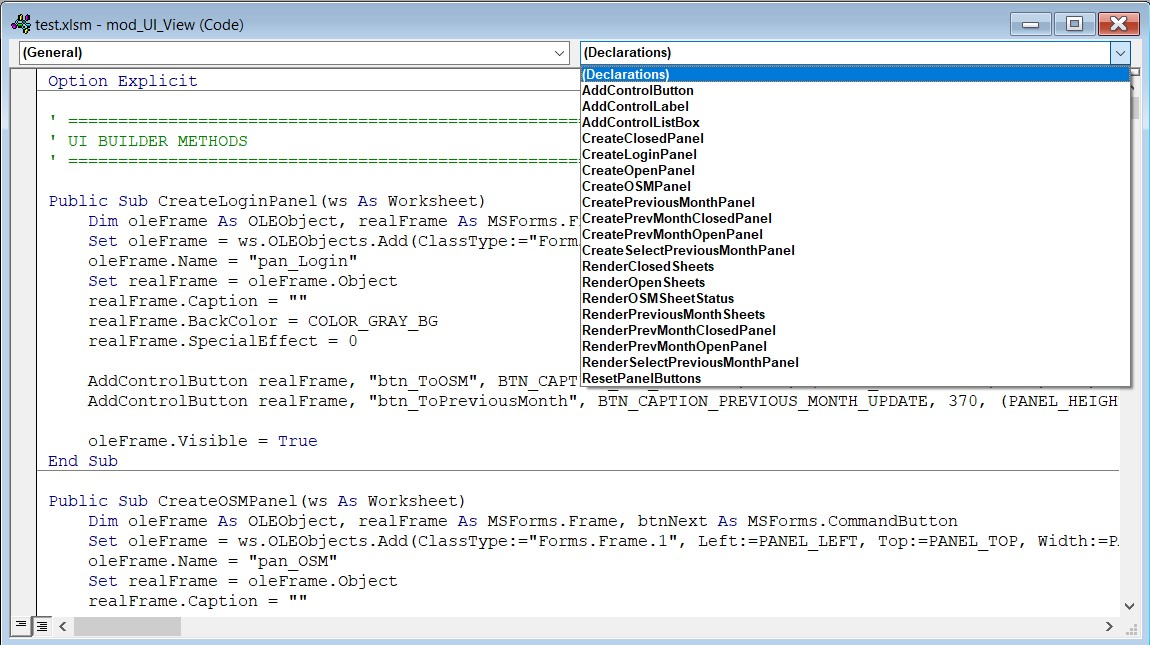
\includegraphics[width=0.88\textwidth, keepaspectratio]{mod_UI_View.jpg}}
    \caption{\texttt{mod\_UI\_View} Modülü Prosedür ve Fonksiyon Dizilimi}
    \label{fig:mod_ui_view_code}
\end{figure}

\vspace{0.2cm}

\textbf{\textcolor{primary}{2. Arayüz Oluşturucuları (UI Builder Methods)}}

Çalışma kitabı ilk açıldığında veya yapılandırma sıfırlandığında, sistemdeki her bir iş akışı paneli (\texttt{Login}, \texttt{OSM}, \texttt{Open}, \texttt{Closed}, \texttt{PreviousMonth}, \texttt{SelectPreviousMonth} vb.) özel oluşturucu prosedürler tarafından inşa edilir. 

Panel yapım aşamasında izlenen standart işlem adımları şunlardır:
\begin{enumerate}\setlength{\itemsep}{0pt}\setlength{\parskip}{1pt}
    \item Aktif sayfada \texttt{OLEObjects.Add} fonksiyonu ile yeni bir \texttt{MSForms.Frame} örneği açılır.
    \item Panelin arka plan rengi, kenarlık stili ve konum parametreleri ayarlanır.
    \item Yardımcı private metotlar (\texttt{AddControlButton}, \texttt{AddControlLabel}, \texttt{AddControlListBox}) kullanılarak panel içerisine gerekli kontrol elemanları yerleştirilir.
    \item Oluşturulan buton referansları bellek kaybolmasını önlemek için \texttt{clsDynamicButton} wrapper sınıfına tescil edilir.
\end{enumerate}

\vspace{0.3cm}

\textbf{\textcolor{primary}{3. Veri Render Yöneticileri (UI Renderer Methods)}}

Kullanıcı paneller arasında geçiş yaptığında veya tarama/güncelleme butonlarına bastığında \texttt{Render*} prosedürleri devreye girer. Bu prosedürler, arka plandaki servislerden dönen dinamik veriyi okur ve \texttt{ListBox} elemanlarını kolon genişliklerine göre biçimlendirerek doldurur.

\newpage
Render sürecinde öne çıkan temel mantıksal mekanizmalar:
\begin{itemize}\setlength{\itemsep}{0pt}\setlength{\parskip}{1pt}
    \item \textbf{Sütun Başlıkları ve Tablo Hizalama:} Her render işleminde \texttt{ListBox.Clear} ile liste sıfırlanır ve ilk satıra sabit tablo başlıkları yüklenir.
    \item \textbf{Otomatik Veri Dönüşümü ve Eşleme:} Veritabanı hücre adresleri (\texttt{D4}, \texttt{K2} vb.) ve ilişkili sayfa isimleri birleştirilerek açıklayıcı metinler (\textit{Örn: D4 (ARIZA)}) halinde listeye aktarılır.
    \item \textbf{Zamanlayıcı ve Otomatik Kilit Mekanizması:} Ekran render edildikten sonra tarama butonlarının aktif kalması ve hatalı çift tıklamaların önlenmesi amacıyla \texttt{Application.OnTime} kullanılarak panel belirli bir süre sonra otomatik kilit durumuna alınır.
    \item \textbf{Boş Satır Tamamlama (Dikey Izgara Düzeni):} Görsel bütünlüğü korumak amacıyla veriler yüklendikten sonra \texttt{ListBox} dikey boyutu dolana kadar boş satır tamamlama döngüsü (\texttt{Do While ListCount < 12}) çalıştırılır.
\end{itemize}

\vspace{0.15cm}

\begin{warningbox}{\faExclamationTriangle\ Arayüz Kararlılığı ve Hata İşleme}
Render işlemleri esnasında geçersiz sayfa yapıları veya silinmiş OLE nesneleri nedeniyle çökme yaşanmaması adına, buton sıfırlayıcı yardımcı prosedürlerde (\texttt{ResetPanelButtons}) yerel hata yönetimi (\texttt{On Error Resume Next}) uygulanmaktadır.
\end{warningbox}

\vspace{0.4cm}

\begin{tcolorbox}[colback=yellow!15,colframe=orange!80!black,leftrule=3.5pt,boxrule=0.4pt,top=5pt,bottom=5pt]
    \textbf{\textcolor{orange!80!black}{\faInfoCircle\ mod\_UI\_View Genel Özet ve Mimari Rolü:}}\\
    \small \texttt{mod\_UI\_View}, uygulamanın tüm görsel bileşenlerini ve tablo ekranlarını kod üzerinden dinamik üreten bir **Grafik Motoru** işlevi görür. Veri işleme mantığını görsel tasarımdan tamamen ayırarak (MVC mimari yaklaşımı), projenin sürdürülebilirliğine ve kolay genişletilebilir bir arayüz yapısına kavuşmasına doğrudan katkı sağlar.
\end{tcolorbox}

\newpage

% ==========================================
% BÖLÜM 4.7: MOD_SERVICES (İŞ MANTIĞI VE VERİ SERVİSLERİ KATMANI)
% ==========================================

\section{\texttt{mod\_Services}}

\texttt{mod\_Services}, uygulamanın tüm veri işleme, hesaplama, veritabanı kesişim adresi bulma, sayfa tarama ve Excel hücre yazma algoritmalarından sorumlu **İş Mantığı Katmanıdır (Business Logic Layer)**. 

Arayüz katmanları (\texttt{mod\_UI\_View}, \texttt{mod\_UI\_Events}) kullanıcı etkileşimlerini yönetip form verilerini toplarken, \texttt{mod\_Services} arka planda verinin doğruluğunu denetler, metrikleri hesaplar ve veritabanı kesişim adreslerine güvenli yazma operasyonlarını yürütür.

Modül içerisinde yüksek işlem performansı ön planda tutulmuştur. Sayfalarda tek tek hücre okumak yerine, veriler belleğe dinamik diziler (\textit{Variant Arrays}) ve hızlı erişimli Sözlük nesneleri (\textit{Scripting.Dictionary}) olarak alınarak işlenir.

Modülün temel fonksiyonel sorumlulukları dört ana kategoride toplanmaktadır:

\begin{itemize}\setlength{\itemsep}{0pt}\setlength{\parskip}{1pt}
    \item \textbf{Çalışma Kitabı ve Sayfa Taramaları:} Kitap içerisindeki tüm sayfaları dolaşarak aktif vaka veya bakım raporlarını tespit eder (\texttt{ScanWorkbookSheets}, \texttt{ScanPreviousMonthSheets}).
    \item \textbf{Tarih ve Dinamik Adres Algoritmaları:} Rapor tarihlerini analiz eder, hedef veritabanı sayfasında ilgili tarih kolonu ile durum satırının kesiştiği hücreyi bulur (\texttt{GetReportDate}, \texttt{FindIntersectCell}).
    \item \textbf{Gelişmiş Metrik Hesaplamaları:} Personel bazlı kapalı vaka sayılarını ve geçmiş ay verilerini dinamik matrislerle hesaplar (\texttt{GetOpenCasesCalculated}, \texttt{GetClosedCasesCalculated}).
    \item \textbf{Veritabanı Yazma Motoru:} Arayüzdeki listelerden gelen verileri süzerek doğrudan veritabanı hücrelerine işler (\texttt{ExecuteDatabaseWrite}, \texttt{ExecutePreviousMonthWrite}).
\end{itemize}

\vspace{0.15cm}

\begin{infobox}{\faCogs\ Performans Odaklı Bellek Yönetimi (In-Memory Data Engine)}
\texttt{CountClosedCasesByPerson} ve \texttt{CountOpenCasesByPerson} gibi fonksiyonlar, çalışma sayfasındaki verileri \texttt{ws.Range.Value} komutuyla tek hamlede RAM üzerindeki çift boyutlu dizilere aktarır. Döngüler bellekte döndüğü için binlerce satırlık veriler milisaniyeler içerisinde işlenir.
\end{infobox}

\vspace{0.3cm}

\textbf{\textcolor{primary}{1. Geliştirme Ortamı ve Modül Yapısı}}

Aşağıdaki ekran görüntüsünde, VBA Geliştirme Ortamı (\textit{VBE}) üzerinde \texttt{mod\_Services} modülünün barındırdığı iş mantığı, tarama, hesaplama ve yardımcı fonksiyonların genel dizilimi gösterilmektedir:

\vspace{0.25cm}

% Resmin Tam Buraya Çakılması İçin Ortamsız Yapı
\begin{center}
    \fboxsep=0pt
    \fboxrule=0.8pt
    \fcolorbox{bordergray}{white}{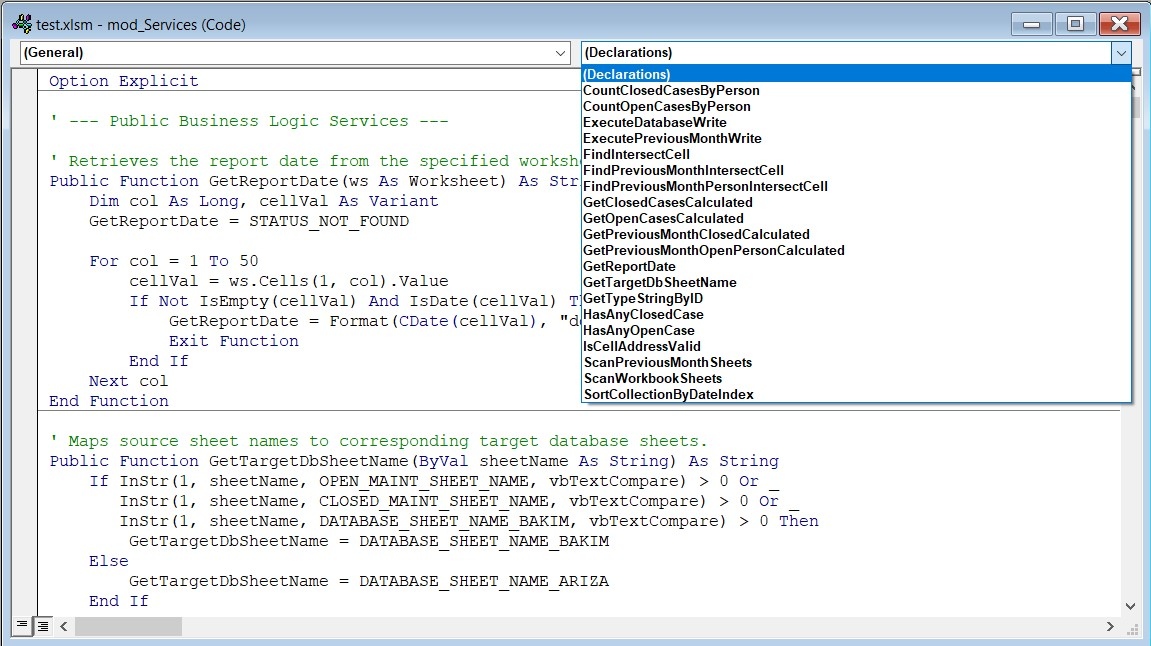
\includegraphics[width=0.85\textwidth, keepaspectratio]{mod_Services.jpg}}
    \captionof{figure}{\texttt{mod\_Services} Modülü Prosedür ve Fonksiyon Dizilimi}
    \label{fig:mod_services_code}
\end{center}

\vspace{0.25cm}

\textbf{\textcolor{primary}{2. Kesişim Adresi Algoritması (FindIntersectCell)}}

Veritabanı sayfalarında aranan tarihe ait sütun ile ilgili durum satırının kesiştiği hücre adresini (\textit{Örn: D4}) dinamik olarak tespit eden temel algoritma aşağıdadır:

\begin{lstlisting}[caption={Dinamik Kesişim Adresi Bulma Fonksiyonu}]
Public Function FindIntersectCell(ByVal dbSheetName As String, ByVal targetDateStr As String, ByVal searchColName As String, ByVal contextText As String) As String
    Dim dbWs As Worksheet, i As Long, tRow As Long, tCol As Long
    FindIntersectCell = STATUS_NOT_FOUND
    
    On Error Resume Next
    Set dbWs = ThisWorkbook.Sheets(dbSheetName)
    On Error GoTo 0
    If dbWs Is Nothing Or Not IsDate(targetDateStr) Then Exit Function
    
    ' 1. Tarih Sutununu Bul
    For i = dbWs.Columns(DB_OSM_DATES_START_COL).Column To dbWs.Columns(DB_OSM_DATES_END_COL).Column
        If IsDate(dbWs.Cells(1, i).Value) Then
            If CDate(dbWs.Cells(1, i).Value) = CDate(targetDateStr) Then tCol = i: Exit For
        End If
    Next i
    
    ' 2. Baglam Satirini Bul (searchColName uzerinde contextText aranir)
    ' . . . (dbLastRow hesaplanarak tRow indeksi tespit edilir)
    
    ' 3. Kesisim Adresini Dondur (Orn: "D4")
    If tRow > 0 And tCol > 0 Then
        FindIntersectCell = dbWs.Cells(tRow, tCol).Address(RowAbsolute:=False, ColumnAbsolute:=False)
    End If
End Function
\end{lstlisting}

\vspace{0.3cm}

\textbf{\textcolor{primary}{3. Personel Bazlı Gruplama ve Hesaplama Metotları}}

Sayfalardaki kapalı vakaları personellere göre gruplarken \texttt{Scripting.Dictionary} yapısı kullanılır. Sayılan değerler \texttt{FindIntersectCell} ile bulunan adreslerle birleştirilerek koleksiyona yüklenir:

\begin{lstlisting}[caption={Kapalı Vakaların Personel Bazlı Hesaplama Mimarisi}]
Public Function GetClosedCasesCalculated() As Collection
    Dim closedCol As New Collection, dict As Object, item As Variant
    Set dict = CreateObject("Scripting.Dictionary")
    
    For Each item In ScanWorkbookSheets()
        If (item(1) = RPT_TYPE_CLOSED_CASE Or item(1) = RPT_TYPE_CLOSED_MAINT) And item(2) <> STATUS_NOT_FOUND Then
            ' Kesisim adresi ile verileri birlestirip koleksiyona ekleme
            dbName = GetTargetDbSheetName(CStr(item(4)))
            For Each key In dict.Keys
                targetCell = FindIntersectCell(dbName, CStr(item(3)), DB_CLOSED_NAME_COL, CStr(key))
                If targetCell <> STATUS_NOT_FOUND And targetCell <> STATUS_NO_DB_SHEET Then
                    closedCol.Add Array(item(4), item(2), item(3), CStr(key), dict(key), targetCell)
                End If
            Next key
            dict.RemoveAll
        End If
    Next item
    Set GetClosedCasesCalculated = SortCollectionByDateIndex(closedCol, 3)
End Function
\end{lstlisting}

\vspace{0.3cm}

\textbf{\textcolor{primary}{4. Güvenli Veritabanı Yazma Motoru}}

Arayüzdeki listelerden okunan güncellenmiş değerler, parantezli sayfa eklerinden (\textit{Örn: D4 (ARIZA)}) ayıklanarak doğrudan veritabanı hücrelerine işlenir:

\begin{lstlisting}[caption={Veritabanı Hücre Yazma Operasyonu}]
Public Function ExecuteDatabaseWrite(lst As MSForms.ListBox, cellColIdx As Long, valColIdx As Long, sheetNameColIdx As Long) As Boolean
    Dim dbWs As Worksheet, i As Long, addr As String, caseVal As Long
    
    For i = 1 To lst.ListCount - 1
        addr = Trim("" & lst.List(i, cellColIdx))
        If InStr(addr, "(") > 0 Then addr = Trim(Split(addr, "(")(0))
        
        If addr <> "" And addr <> STATUS_NOT_FOUND And addr <> STATUS_NO_DB_SHEET Then
            targetDbName = GetTargetDbSheetName(Trim("" & lst.List(i, sheetNameColIdx)))
            Set dbWs = ThisWorkbook.Sheets(targetDbName)
            
            If Not dbWs Is Nothing Then
                caseVal = Val("" & lst.List(i, valColIdx))
                dbWs.Range(addr).Value = caseVal
            End If
        End If
    Next i
    ExecuteDatabaseWrite = True
End Function
\end{lstlisting}

\vspace{0.15cm}

\begin{warningbox}{\faExclamationTriangle\ Hata Önleme ve Hücre Doğrulama}
Yazma operasyonları öncesinde \texttt{IsCellAddressValid} fonksiyonu çalıştırılarak hücre adresinin varlığı teyit edilir. Olası sayfa bulunamama veya hatalı adres durumlarında yazma işlemi iptal edilerek kullanıcı bilgilendirilir.
\end{warningbox}

\vspace{0.4cm}

\begin{tcolorbox}[colback=yellow!15,colframe=orange!80!black,leftrule=3.5pt,boxrule=0.4pt,top=5pt,bottom=5pt]
    \textbf{\textcolor{orange!80!black}{\faInfoCircle\ mod\_Services Genel Özet ve Mimari Rolü:}}\\
    \small \texttt{mod\_Services}, uygulamanın **Çekirdek Veri Motorudur**. Arayüz bileşenlerinden bağımsız çalışır, girdi verilerini dönüştürür, dinamik adres kesişimlerini hesaplar ve Excel hücre düzeyindeki yazma/okuma operasyonlarını yüksek performansla gerçekleştirir.
\end{tcolorbox}
% ==========================================
% BÖLÜM 5: GELİŞTİRİCİ VE KATKI SAĞLAMA REHBERİ
% ==========================================
\chapter{Geliştirici Rehberi}

Bu bölüm, uygulamanın gelecekte yeni özelliklerle genişletilmesi, değişen kurum içi rapor yapılarına kolayca adapte edilmesi, veritabanı yapılarının güncellenmesi ve mimariye yeni dinamik panellerin eklenmesi süreçlerinde takip edilmesi gereken standartları detaylandırmaktadır.

Uygulamanın sürdürülebilir kalması için geliştiricilerin aşağıda yer alan 4 temel senaryoyu ve katmanlı mimari kurallarını adım adım uygulaması büyük önem taşımaktadır.

\vspace{0.4cm}

% ==========================================
% SENARYO 1: RAPOR BİÇİMİ / SÜTUN DEĞİŞİKLİĞİ
% ==========================================
\section{Senaryo 1: Gelen Rapor Biçimi veya Sütun Yapısı Değişirse}

Sistemdeki en büyük mimari avantaj, kod satırlarına sert biçimde yazılmış (\textit{Hardcoded}) sayfa/sütun isimlerinin veya dinamik metinlerin bulunmamasıdır. Kurum içi raporlarda sütun harfleri, sayfa isimleri veya vaka durum başlıkları değiştiğinde izlenecek adımlar aşağıda detaylandırılmıştır:

\vspace{0.2cm}

\textbf{\textcolor{primary}{1. Yapılandırma Modülüne (\texttt{mod\_Config}) Erişin:}}
\begin{itemize}\setlength{\itemsep}{2pt}
    \item Klavyeden \textbf{\texttt{Alt + F11}} kısayol tuşlarına basarak VBA Editörüne girin ve sol menüden \texttt{mod\_Config} modülünü açın.
    \item Tüm sistem sabitlerinin kategorize edildiği bu alanda sadece ilgili sabit değerini güncelleyin.
\end{itemize}

\vspace{0.15cm}

\textbf{\textcolor{primary}{2. Sütun Harflerini ve Hücre Adreslerini Revize Edin:}}
Rapor sayfalarındaki sütun yerleri değiştiğinde \texttt{mod\_Config} içerisindeki ilgili harfleri güncelleyin:
\begin{lstlisting}[caption={Sütun Sabitlerinin Güncellenmesi}]
' Eski: Public Const ALL_CASES_STATUS_COL As String = "AF"
' Yeni Sütun Konumu:
Public Const ALL_CASES_STATUS_COL As String = "AG"
Public Const ALL_CASES_CLOSE_DATE_COL As String = "X"
\end{lstlisting}

\vspace{0.15cm}

\textbf{\textcolor{primary}{3. Durum Metinlerini ve Kelime Filtrelerini Genişletin:}}
Sisteme yeni bir vaka durumu eklendiyse veya durum kelimeleri değiştiyse (Örn: "Çözüldü" yerine "Tamamlandı" veya "İşlemde" yerine "Devam Ediyor" geldiyse); sabit listelerine yeni kelimeyi virgülle ekleyin:
\begin{lstlisting}[caption={Geçerli Durum Sabitlerinin Güncellenmesi}]
Public Const VALID_CLOSED_STATUSES As String = "Çözüldü,Kapandı,Kapalı,Cozuldu,KAPANDI,KAPALI,Tamamlandı,TAMAMLANDI"
Public Const VALID_OPEN_STATUSES   As String = "Açık,Atandı,Beklemede,İşlemde,Acik,Atandi,Islemde,Devam Ediyor"
\end{lstlisting}

\vspace{0.15cm}

\textbf{\textcolor{primary}{4. İş Mantığı Katmanını Koruyun:}}
Sütun veya durum ismi değişikliklerinde \texttt{mod\_Services} içerisindeki algoritmik kodlara dokunmanıza kesinlikle gerek yoktur; arka plan servisleri dinamik olarak yenilenen bu sabitleri okuyarak kesişim hücrelerini hesaplayacaktır.

\newpage

% ==========================================
% SENARYO 2: ARAYÜZE YENİ PANEL EKLEME
% ==========================================
\section{Senaryo 2: Arayüze Yeni Bir Panel Ekleme (\texttt{CreateYEPYENIPanel})}

Login paneline veya genel iş akışına yepyeni bir işlem ekranı (Panel) dahil edilmek istendiğinde projenin Katmanlı Mimarisi sırasıyla takip edilerek adımlar yürütülür:

\vspace{0.2cm}

\textbf{\textcolor{primary}{1. Adım: Sabit ve Görsel Metin Tanımlamaları (\texttt{mod\_Config})}}
\texttt{mod\_Config} modülünde yeni eklenen panelin başlığı ve buton yazıları için sabitler tanımlanır:
\begin{lstlisting}[caption={Yeni Panel Sabitlerinin Tanımlanması}]
Public Const LBL_YEPYENI_PANEL_TITLE As String = "YEPYENİ ÖZEL ANALİZ PANELİ"
Public Const BTN_CAPTION_TO_YEPYENI  As String = "YEPYENİ ANALİZ"
\end{lstlisting}

\vspace{0.2cm}

\textbf{\textcolor{primary}{2. Adım: Panel Yapıcısı ve Çizim Prosedürü (\texttt{mod\_UI\_View})}}
\texttt{mod\_UI\_View} modülü içerisine yeni OLE Frame bileşenini ve içerisindeki kontrol elemanlarını (Label, Button, ListBox) çizen \texttt{CreateYEPYENIPanel} prosedürü yazılır:
\begin{lstlisting}[caption={CreateYEPYENIPanel Çizim Prosedürü}]
Public Sub CreateYEPYENIPanel(ws As Worksheet)
    Dim oleFrame As OLEObject, realFrame As MSForms.Frame
    Set oleFrame = ws.OLEObjects.Add(ClassType:="Forms.Frame.1", Left:=PANEL_LEFT, Top:=PANEL_TOP, Width:=PANEL_WIDTH, Height:=PANEL_HEIGHT)
    oleFrame.Name = "pan_YEPYENIPanel"
    Set realFrame = oleFrame.Object
    realFrame.Caption = ""
    realFrame.BackColor = COLOR_GRAY_BG
    
    AddControlLabel realFrame, "lbl_YepyeniTitle", LBL_YEPYENI_PANEL_TITLE, 40, 20
    AddControlListBox realFrame, "lst_YepyeniStatus", 4, "150;100;120;150"
    AddControlButton realFrame, "btn_BackToLogin", BTN_CAPTION_BACK, 40, 260, 120, 35, COLOR_RED
    AddControlButton realFrame, "btn_UpdateYepyeni", BTN_CAPTION_UPDATE, 380, 260, 120, 35, COLOR_WHITE, &H333333
    oleFrame.Visible = False
End Sub
\end{lstlisting}

\vspace{0.2cm}

\textbf{\textcolor{primary}{3. Adım: Sistem Kaydı ve Navigasyon Entegrasyonu (\texttt{mod\_UI\_Manager})}}
\begin{itemize}\setlength{\itemsep}{2pt}
    \item \texttt{BuildNavigationSystem} prosedürüne \texttt{mod\_UI\_View.CreateYEPYENIPanel ws} çağrısı eklenir.
    \item \texttt{SwitchTo} prosedüründeki panel gizleme alanına \texttt{ws.OLEObjects("pan\_YEPYENIPanel").Visible = False} satırı ve \texttt{Select Case} bloğuna \texttt{"YEPYENIPanel"} seçeneği dahil edilir.
\end{itemize}

\vspace{0.2cm}

\textbf{\textcolor{primary}{4. Adım: Olay Dinleyici ve Yönlendirme Katmanı (\texttt{clsDynamicButton} \& \texttt{mod\_UI\_Events})}}
\begin{itemize}\setlength{\itemsep}{2pt}
    \item \texttt{clsDynamicButton} sınıf modülündeki \texttt{Select Case parentFrame.Name} kontrolüne \texttt{Case "pan\_YEPYENIPanel": mod\_UI\_Events.HandleYEPYENIPanelEvents DynamicButton.Name, parentFrame} satırı eklenir.
    \item \texttt{mod\_UI\_Events} modülüne tıklamaları yöneten \texttt{HandleYEPYENIPanelEvents} prosedürü yazılır.
\end{itemize}

\newpage

% ==========================================
% SENARYO 3: YENİ HESAPLAMA SERVİSİ EKLEME
% ==========================================
\section{Senaryo 3: Yeni Bir İş Mantığı veya Hesaplama Servisi Ekleme}

Uygulamaya yeni bir hesaplama, metrik analizi veya özel rapor tarama özelliği eklenmesi gerektiğinde izlenecek mimari adımlar:

\vspace{0.3cm}

\textbf{\textcolor{primary}{1. Servis Fonksiyonunu \texttt{mod\_Services} İçinde Kurgulayın:}}
Tüm veri işleme, filtreleme ve matris kesişim adresi bulma mantığını arayüz görsel kodlarından tamamen bağımsız olarak bu modülde bir \texttt{Function} olarak yazın:
\begin{lstlisting}[caption={Yeni Hesaplama Servis Fonksiyonu Örneği}]
Public Function GetYepyeniCalculatedData() As Collection
    Dim results As New Collection, ws As Worksheet
    ' ... Veri tarama ve Scripting.Dictionary ile gruplama adimlari ...
    Set GetYepyeniCalculatedData = results
End Function
\end{lstlisting}

\vspace{0.2cm}

\textbf{\textcolor{primary}{2. Bellek İçi (In-Memory) Diziler Kullanın:}}
Excel hücrelerini döngü ile tek tek gezmek işlem hızını düşürür. Bunun yerine verileri tek hamlede \texttt{Variant} dizisine veya \texttt{Scripting.Dictionary} nesnesine çekerek RAM üzerinde işleyin:
\begin{lstlisting}[caption={RAM Üzerinde Hızlı Veri İşleme}]
Dim dataArray As Variant
dataArray = ws.Range("A2:Z1000").Value ' Tek seferde RAM'e alma
' dataArray(i, j) uzerinden milisaniyeler icinde sorgulama
\end{lstlisting}

\vspace{0.2cm}

\textbf{\textcolor{primary}{3. Sonucu Arayüz Katmanında Render Edin:}}
Hesaplanan sonuçları bir \texttt{Collection} veya dizi olarak döndürün, ardından \texttt{mod\_UI\_View} içindeki \texttt{RenderYEPYENIPanel} prosedürü ile \texttt{ListBox} elemanına bağlayın:
\begin{lstlisting}[caption={ListBox Veri Bağlama (Rendering)}]
Public Sub RenderYEPYENIPanel(realFrame As MSForms.Frame)
    Dim lst As MSForms.ListBox, data As Collection, item As Variant
    Set lst = realFrame.Controls("lst_YepyeniStatus")
    lst.Clear
    Set data = mod_Services.GetYepyeniCalculatedData()
    For Each item In data
        lst.AddItem
        lst.List(lst.ListCount - 1, 0) = item(0)
    Next item
End Sub
\end{lstlisting}

\vspace{0.3cm}

\begin{infobox}{\faSitemap\ Servis Mimarisinin Avantajı}
İş mantığı servis fonksiyonunda kurgulandığı için, gelecekte Excel arayüzü değişse bile \texttt{GetYepyeniCalculatedData} fonksiyonuna dokunulmadan farklı mecralarda tekrar kullanılabilir (Reusability).
\end{infobox}

\newpage

% ==========================================
% SENARYO 4: VERİTABANI/SAYFA EKLEME & MİMARİ KURALLAR
% ==========================================
\section{Senaryo 4: Yeni Veritabanı Çalışma Sayfası Ekleme ve Geliştirme Kuralları}

Sisteme \texttt{ARIZA} ve \texttt{BAKIM} dışında örneğin \texttt{KALITE} veya \texttt{LOJISTIK} adında 3. bir veritabanı sayfası ekleneceği zaman izlenecek süreçler ve uyulması gereken katı geliştirme kuralları şunlardır:

\vspace{0.3cm}

\textbf{\textcolor{primary}{1. Veritabanı Eşleme Fonksiyonunu Güncelleyin:}}
\texttt{mod\_Services} modülündeki \texttt{GetTargetDbSheetName} fonksiyonuna yeni sayfa koşulunu ekleyin:
\begin{lstlisting}[caption={Hedef Veritabanı Eşleme Güncellemesi}]
Public Function GetTargetDbSheetName(ByVal sheetName As String) As String
    If InStr(1, sheetName, "KALITE", vbTextCompare) > 0 Then
        GetTargetDbSheetName = "KALITE"
    ElseIf InStr(1, sheetName, "BAKIM", vbTextCompare) > 0 Then
        GetTargetDbSheetName = DATABASE_SHEET_NAME_BAKIM
    Else
        GetTargetDbSheetName = DATABASE_SHEET_NAME_ARIZA
    End If
End Function
\end{lstlisting}

\vspace{0.2cm}

\textbf{\textcolor{primary}{2. Yeni Veritabanı Sayfa Yapısını Oluşturun:}}
\begin{itemize}\setlength{\itemsep}{2pt}
    \item Sayfanın 1. satırına takip edilecek tarihleri \texttt{dd.mm.yyyy} formatında yerleştirin.
    \item B sütununa (\texttt{B} kolonu) personel/vaka isimlerini yazın.
    \item \textbf{"AÇIK VAKA SAYISI"} ve \textbf{"KAPALI VAKA SAYISI"} arama başlıklarını ilgili satırlara ekleyin.
\end{itemize}

\vspace{0.3cm}

\begin{warningbox}{\faExclamationTriangle\ Katı Kodlama Standartları ve Kalite Kuralları}
Geliştiricilerin kod tabanına müdahale ederken uymakla yükümlü olduğu temel kurallar:
\begin{itemize}\setlength{\itemsep}{2pt}
    \item \textbf{Değişken Bildirimi:} Eklenen her yeni modülün ve sınıfın en başında mutlaka \texttt{Option Explicit} ifadesi yer almalıdır.
    \item \textbf{Hücre Bazlı Döngü Yasağı:} Çalışma sayfası hücreleri üzerinde tek tek \texttt{For Each cell In Range} döngüsü kurulmamalı; veriler belleğe (\texttt{Variant Array} / \texttt{Scripting.Dictionary}) alınarak milisaniyeler seviyesinde işlenmelidir.
    \item \textbf{Bellek Güvenliği:} Dinamik oluşturulan her bir \texttt{MSForms.CommandButton} nesnesi, bellek kayıplarını ve tıklama hatalarını önlemek için merkezi \texttt{ButtonCollection} koleksiyonuna eklenmelidir.
\end{itemize}
\end{warningbox}

\vspace{0.3cm}

\begin{tcolorbox}[colback=yellow!15,colframe=orange!80!black,leftrule=3.5pt,boxrule=0.4pt,top=5pt,bottom=5pt]
    \textbf{\textcolor{orange!80!black}{\faInfoCircle\ Özet ve Katkı Yaklaşımı:}}\\
    \small Bu proje, Modüler Katmanlı Mimari (Layered Architecture) ve MVC (Model-View-Controller) prensipleri doğrultusunda inşa edilmiştir. Yapılacak tüm geliştirmelerde iş mantığı (\texttt{mod\_Services}), görünüm (\texttt{mod\_UI\_View}) ve olay yönlendirme (\texttt{mod\_UI\_Events}) katmanlarının kesinlikle birbirinden ayrık tutulması projenin sürdürülebilirliği için şarttır.
\end{tcolorbox}

\newpage
\chapter{Sonuç}
başak abla selam

\end{document}